


\documentclass[a4paper,11pt]{article}
%\pdfoutput=1 % if your are submitting a pdflatex (i.e. if you have
             % images in pdf, png or jpg format)
\usepackage{jheppub} % for details on the use of the package, please
                     % see the JHEP-author-manual
\usepackage[T1]{fontenc} % if needed
\usepackage{booktabs}

\usepackage{slashed}
%\usepackage{subfigure}
\usepackage{xspace}
\usepackage{booktabs}
%% %simple case: 2 authors, same institution
%% \author{A. Uthor}
%% \author{and A. Nother Author}
%% \affiliation{Institution,\\Address, Country}

\begin{document}
\title{\boldmath Status of the Fittino-ScyNet-SModelS Project}

\author[a]{Federico Ambrogi}
\affiliation[a]{University of Vienna, Institut  f\"ur Meteorologie und Geophysik,  Althanstraße 14 (UZA II), 1090 Wien}
% e-mail addresses: one for each author, in the same order as the authors\emailAdd{federico.ambrogi@oeaw.ac.at}
\emailAdd{federico.ambrogi88@gmail.com}

\maketitle




\newcommand{\MG}{\texttt{MadGraph5\_aMC@NLO}}

\newcommand{\jmet}{ $3jet+E_T^{miss}$ }

\newcommand{\SMO}{ \texttt{SModelS}}
\newcommand{\FastLim}{ \texttt{FastLim}}


\section*{Abstract}


\section{Introduction}

Thsi document summarizes the current status of the project. In addition, the results from a previous (unpublished) work are shown, since they are directly correlated and the current production of the Efficiency Maps (EM) is indeed based on those. 







\section{Previous Results: the ATLAS pMSSM-19 }
In this Section I summarize briefly the outcome of previous studies that I performed (or that I took part in), which are based on the work from ATLAS \cite{} regarding the Run1 interpretation of SUSY searches within the pMSSM-19 work. Main key points of our \SMO~analysis:
\begin{itemize}
	\item we used the same SLHA points from ATLAS \
	\item ATLAS gives information if the point is excluded or not (by their full recast of analyses) \
	\item we could compare if a point could be excluded also by means of simplified models \
	\item we could reach up to 55 or 63$\%$ exclusion only (see Fig. \ref{smo_paper_histo} ) \
	\item the database included official results, but also EM I produced, and EM produced by \FastLim~ \
	\item we studied the most relevant missing topologies (see Fig. \ref{smo_paper_missing} ) 
\end{itemize}

\\

The extension of this study was part of my thesis, which focussed on two points:
\begin{enumerate}
\item of all the results included (i.e. of all the simplified model results in the database), which ones are \textbf{*really*} contribute to exclude at least a decent number of points? \ 
\item can I use this information to choose smartly which EM to create and for which analysis, without guessing efficiencies "a priori" ?
\end{enumerate}
\\

These two are discussed briefly in the following.

\begin{figure}[!]
	\begin{center}
		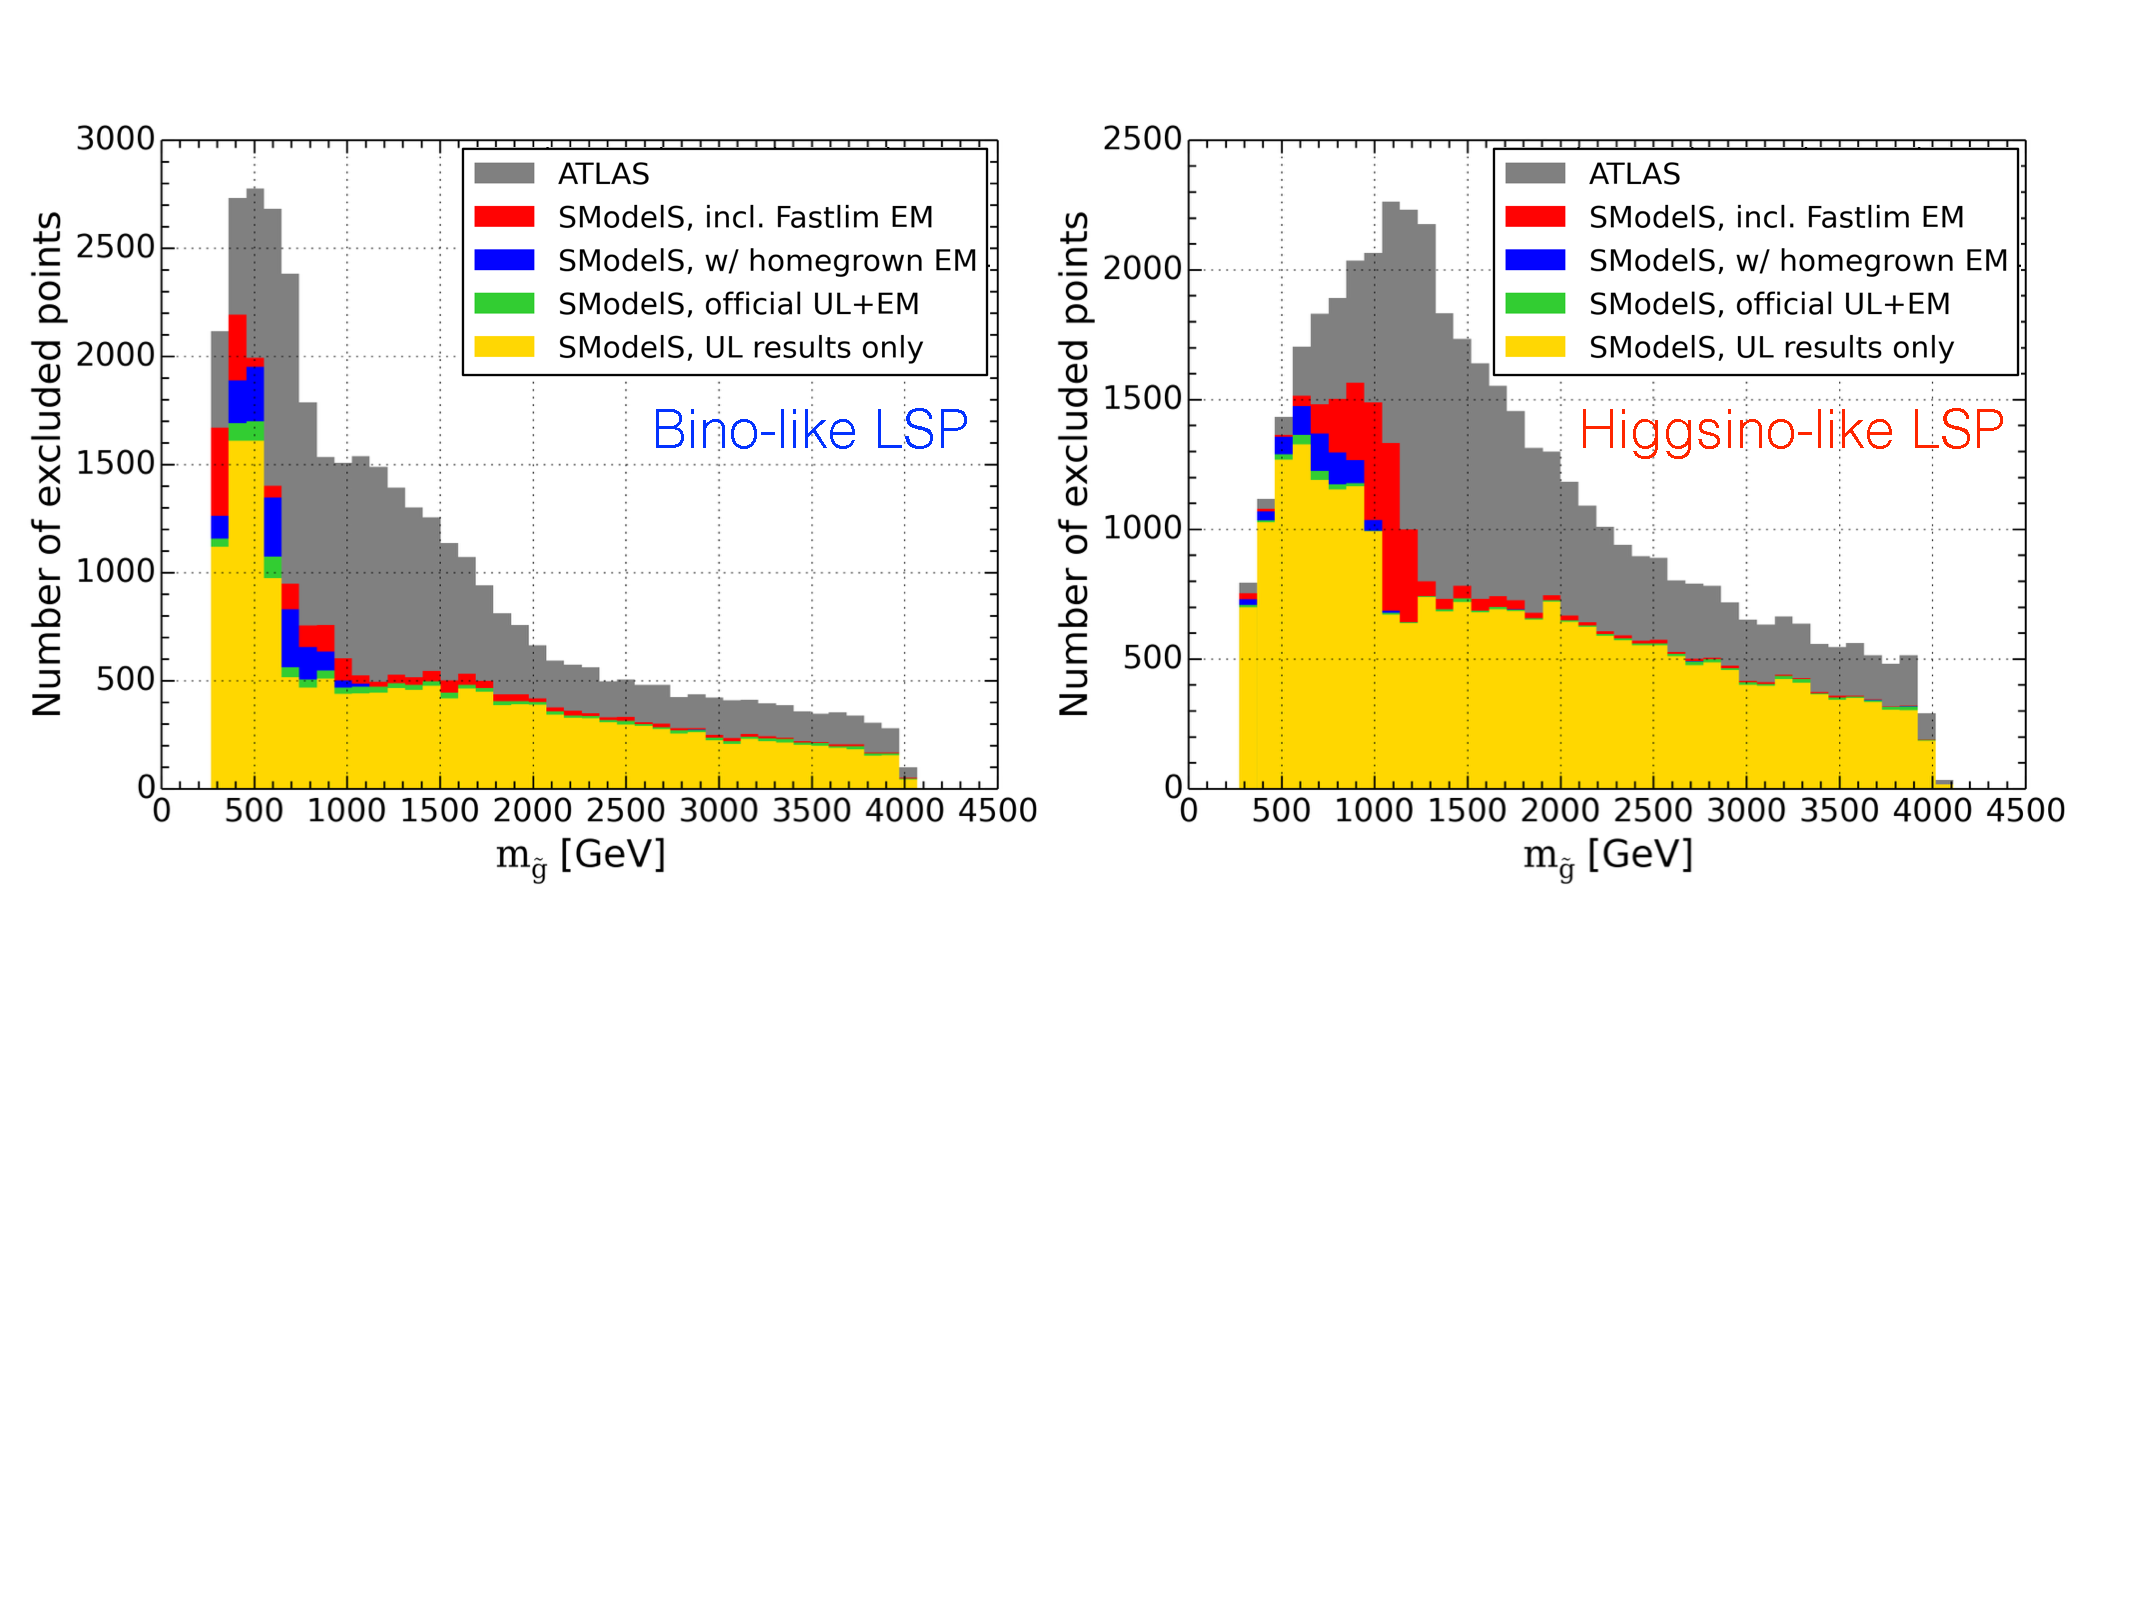
\includegraphics[width=1\textwidth]{Fig/SMO_Paper/Histo_paper.pdf}
	\end{center}
	\caption{Distribution of excluded points using all the results implemented int the \SMO~database, including \fastlim~ results. }
	\label{smo_paper_histo}
\end{figure}


\begin{figure}[!b]
	\centering
	\subfigure
	{ 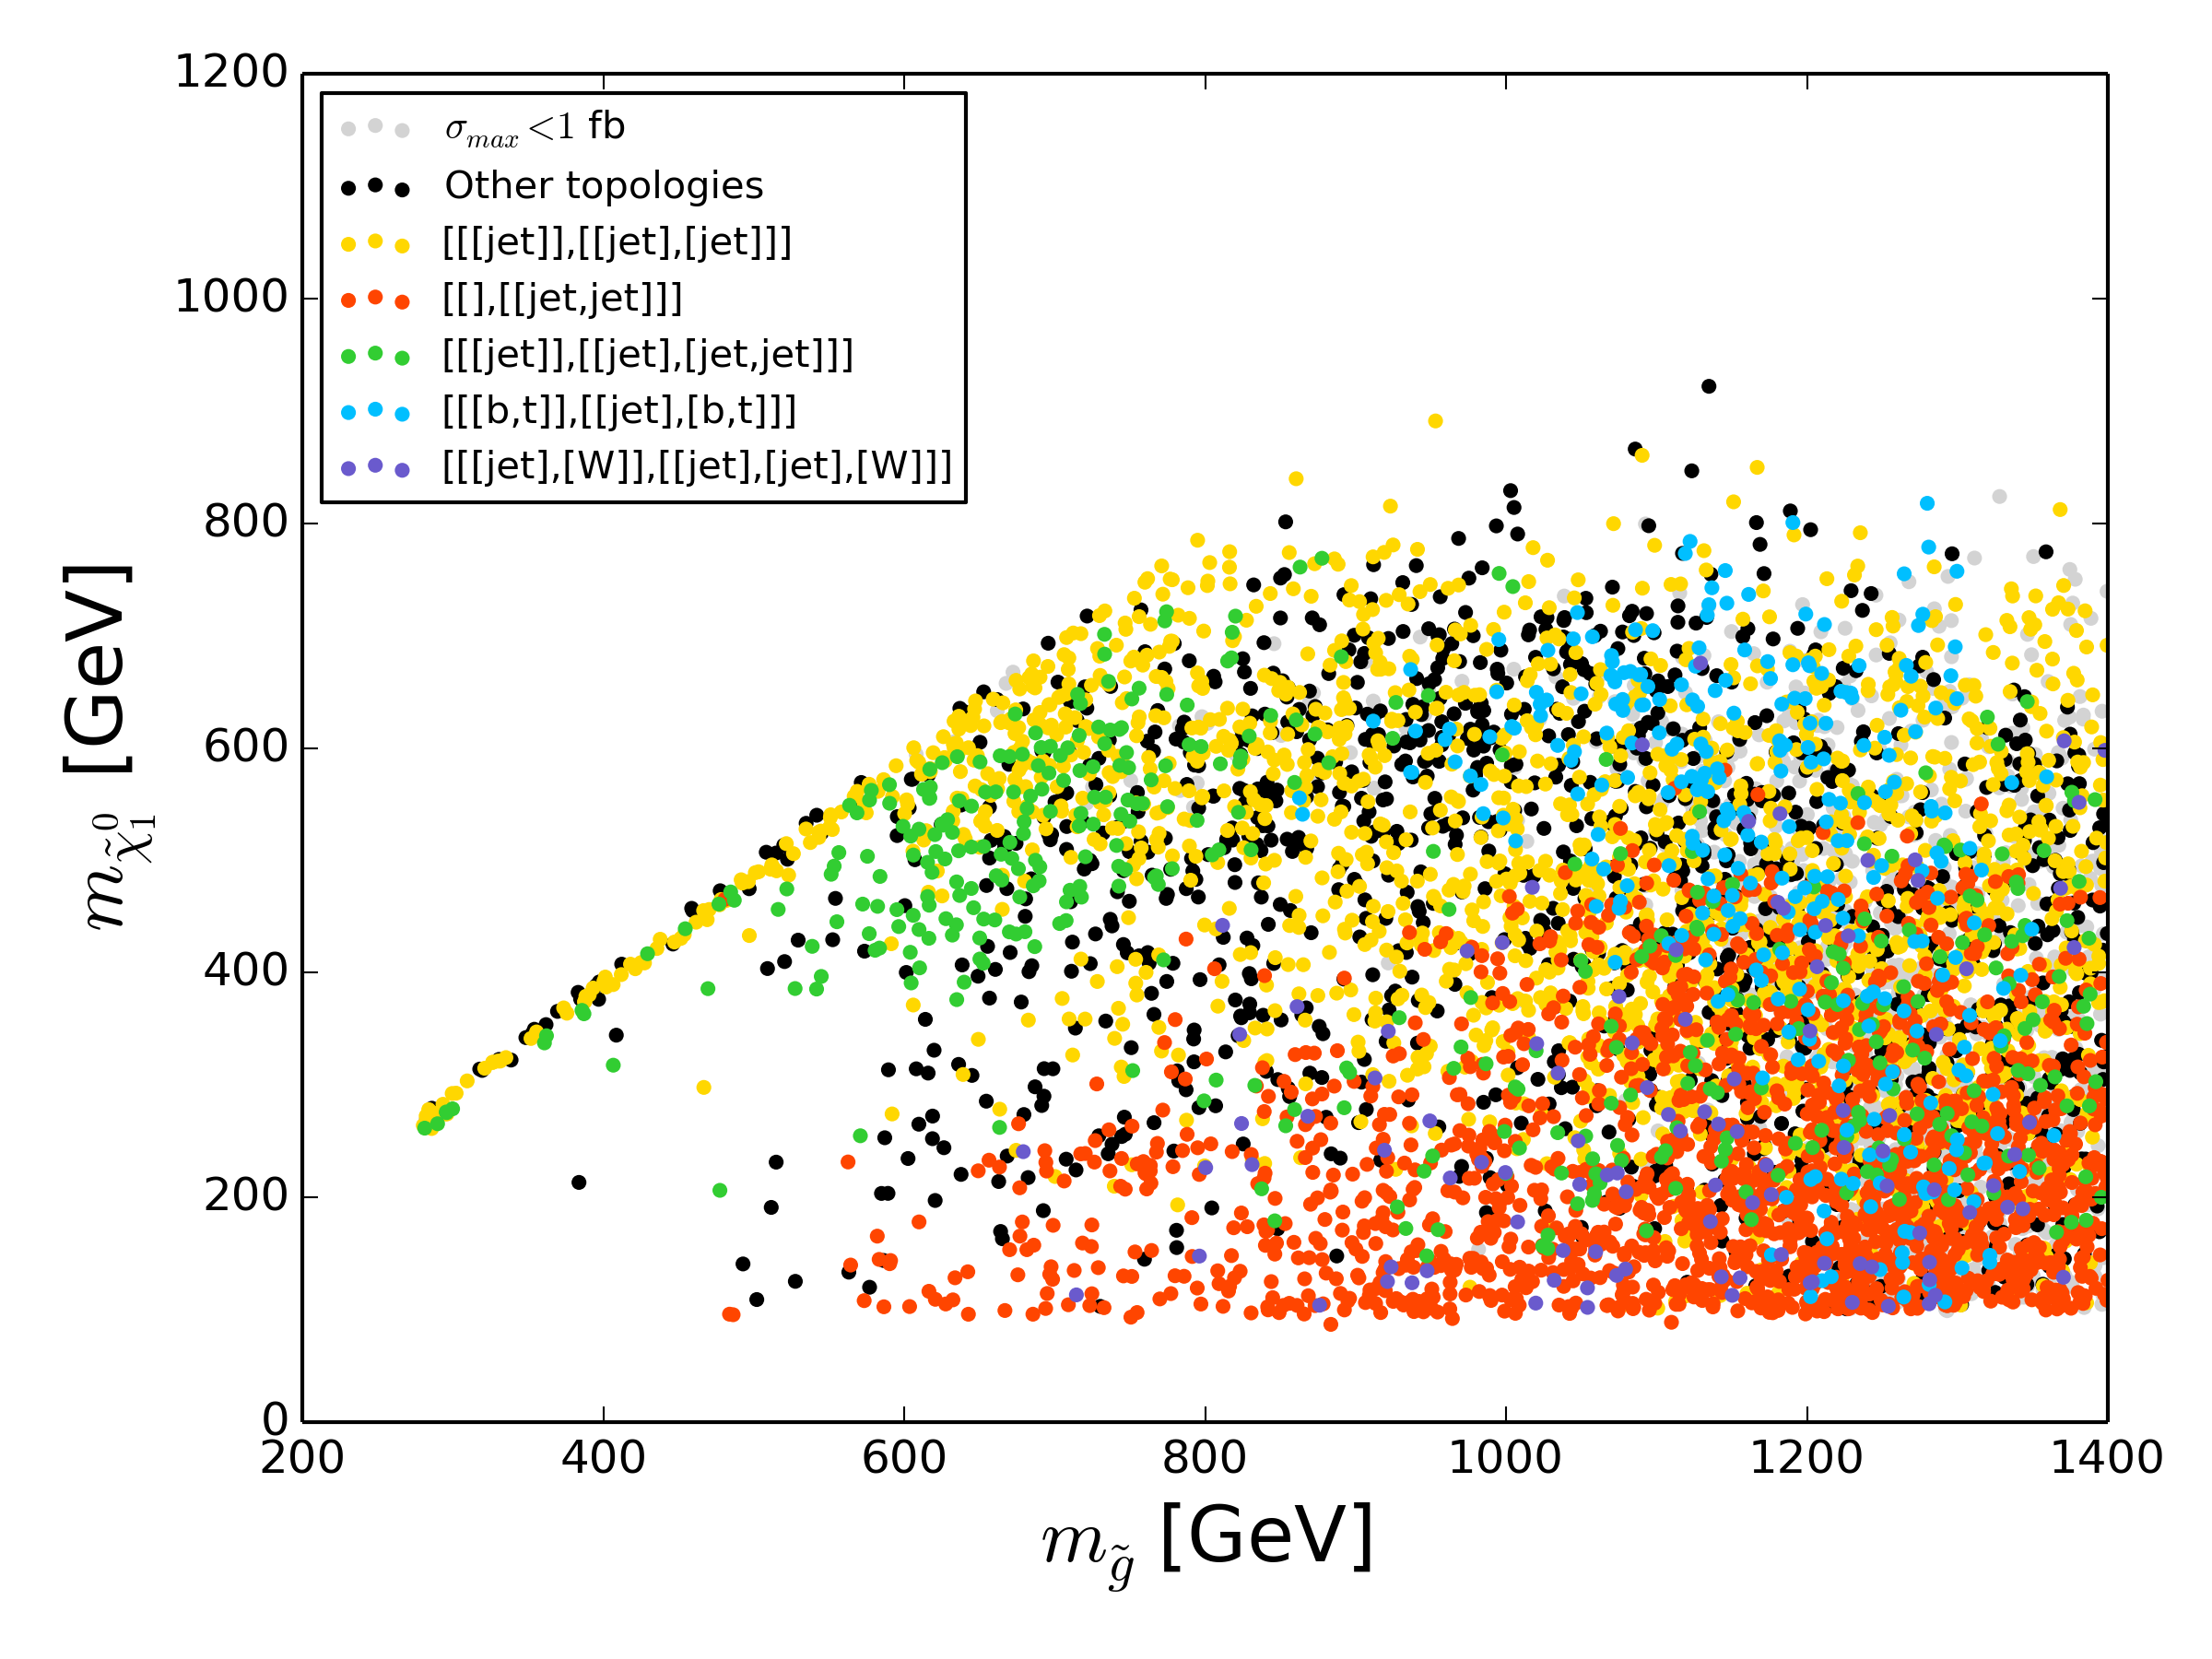
\includegraphics[width=0.49\textwidth]{Fig/SMO_Paper/MissingTopo_HiggsinoLSP.png}}
	\subfigure
	{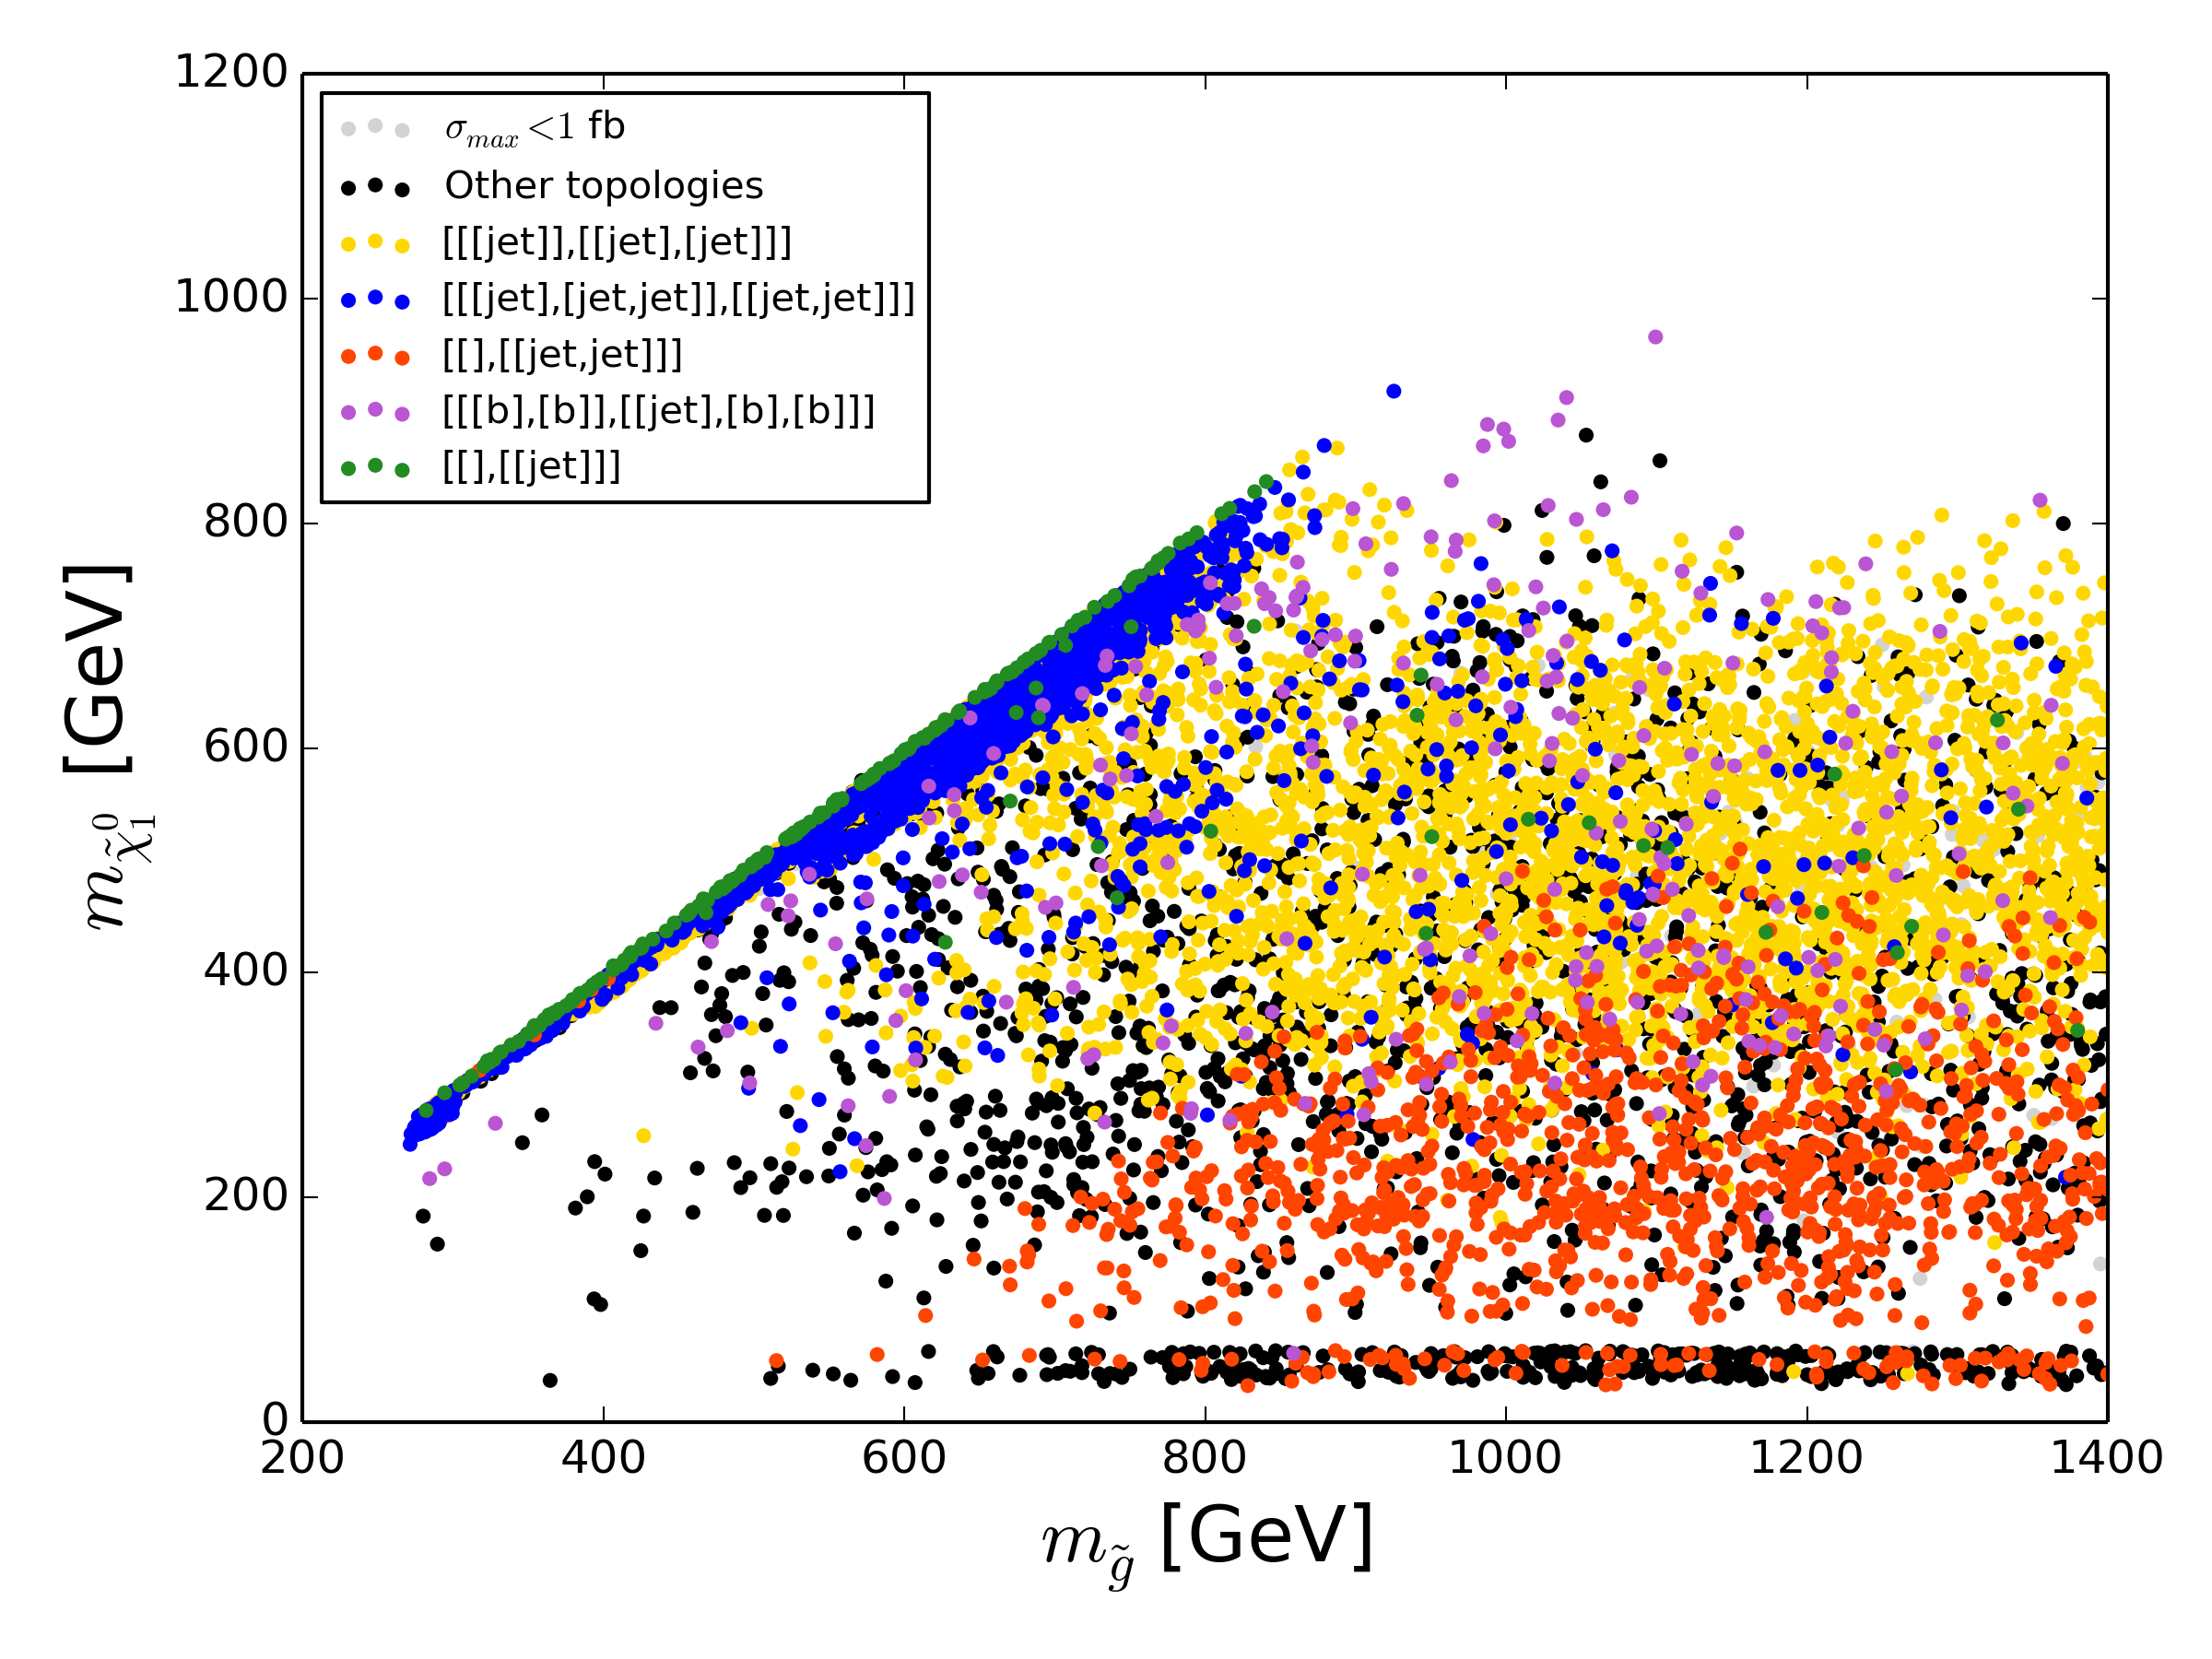
\includegraphics[width=0.49\textwidth]{Fig/SMO_Paper/MissingTopo_BinoLSP.png}}
	\caption{Moste relevant missing topologies (ordered by frequency). Note the \jmet~ topology, most frequent in both cases.}
	\label{smo_paper_missing}
\end{figure}


\clearpage
\section{What excludes what?}\label{ATLAS047}
After checking analysis by analysis, simplified model by simplified model, briefly the conclusion is that the most constraining simplified model results is a CMS upper limit result for the T2 topology (squark production and direct decay), in general, this T2 is efficiently constraining the pMSSM alone, without the need of model combination (with EM). 
\\

However, another aspect I wanted to clarify was the impact of \FastLim~ results, for two reasons. The first one is that the \FastLim~ results contain many different EMs results for the same analysis, so that you can efficiently combine different signals. The second is that the simplified models that they provide results for are "original", and such results cannot be found in official results. (Note that their models focused on natural SUSY scenarios, but also apply to the pMSSM as well in general).
Fig. \ref{fastlim} shows the points excluded by the analysis ATLAS-CONF-2013-047 (i.e. the analysis superseded by ATLAS-SUSY-2013-02 mentioned above). The colours indicate the topologies that give the highest "best" r-value, or the "2nd-best" r-values, or in another words, they tell which model, contributing to the EMs combination, give the highest $\sigma \times BR$. Note that considering the topologies carrying the best r-value might not be enough to reach r-value$>$1, i.e. the r-values of each single simplified model is not necessarily $>$1. 


\begin{figure}[!b]
	\centering
	\subfigure
	{ 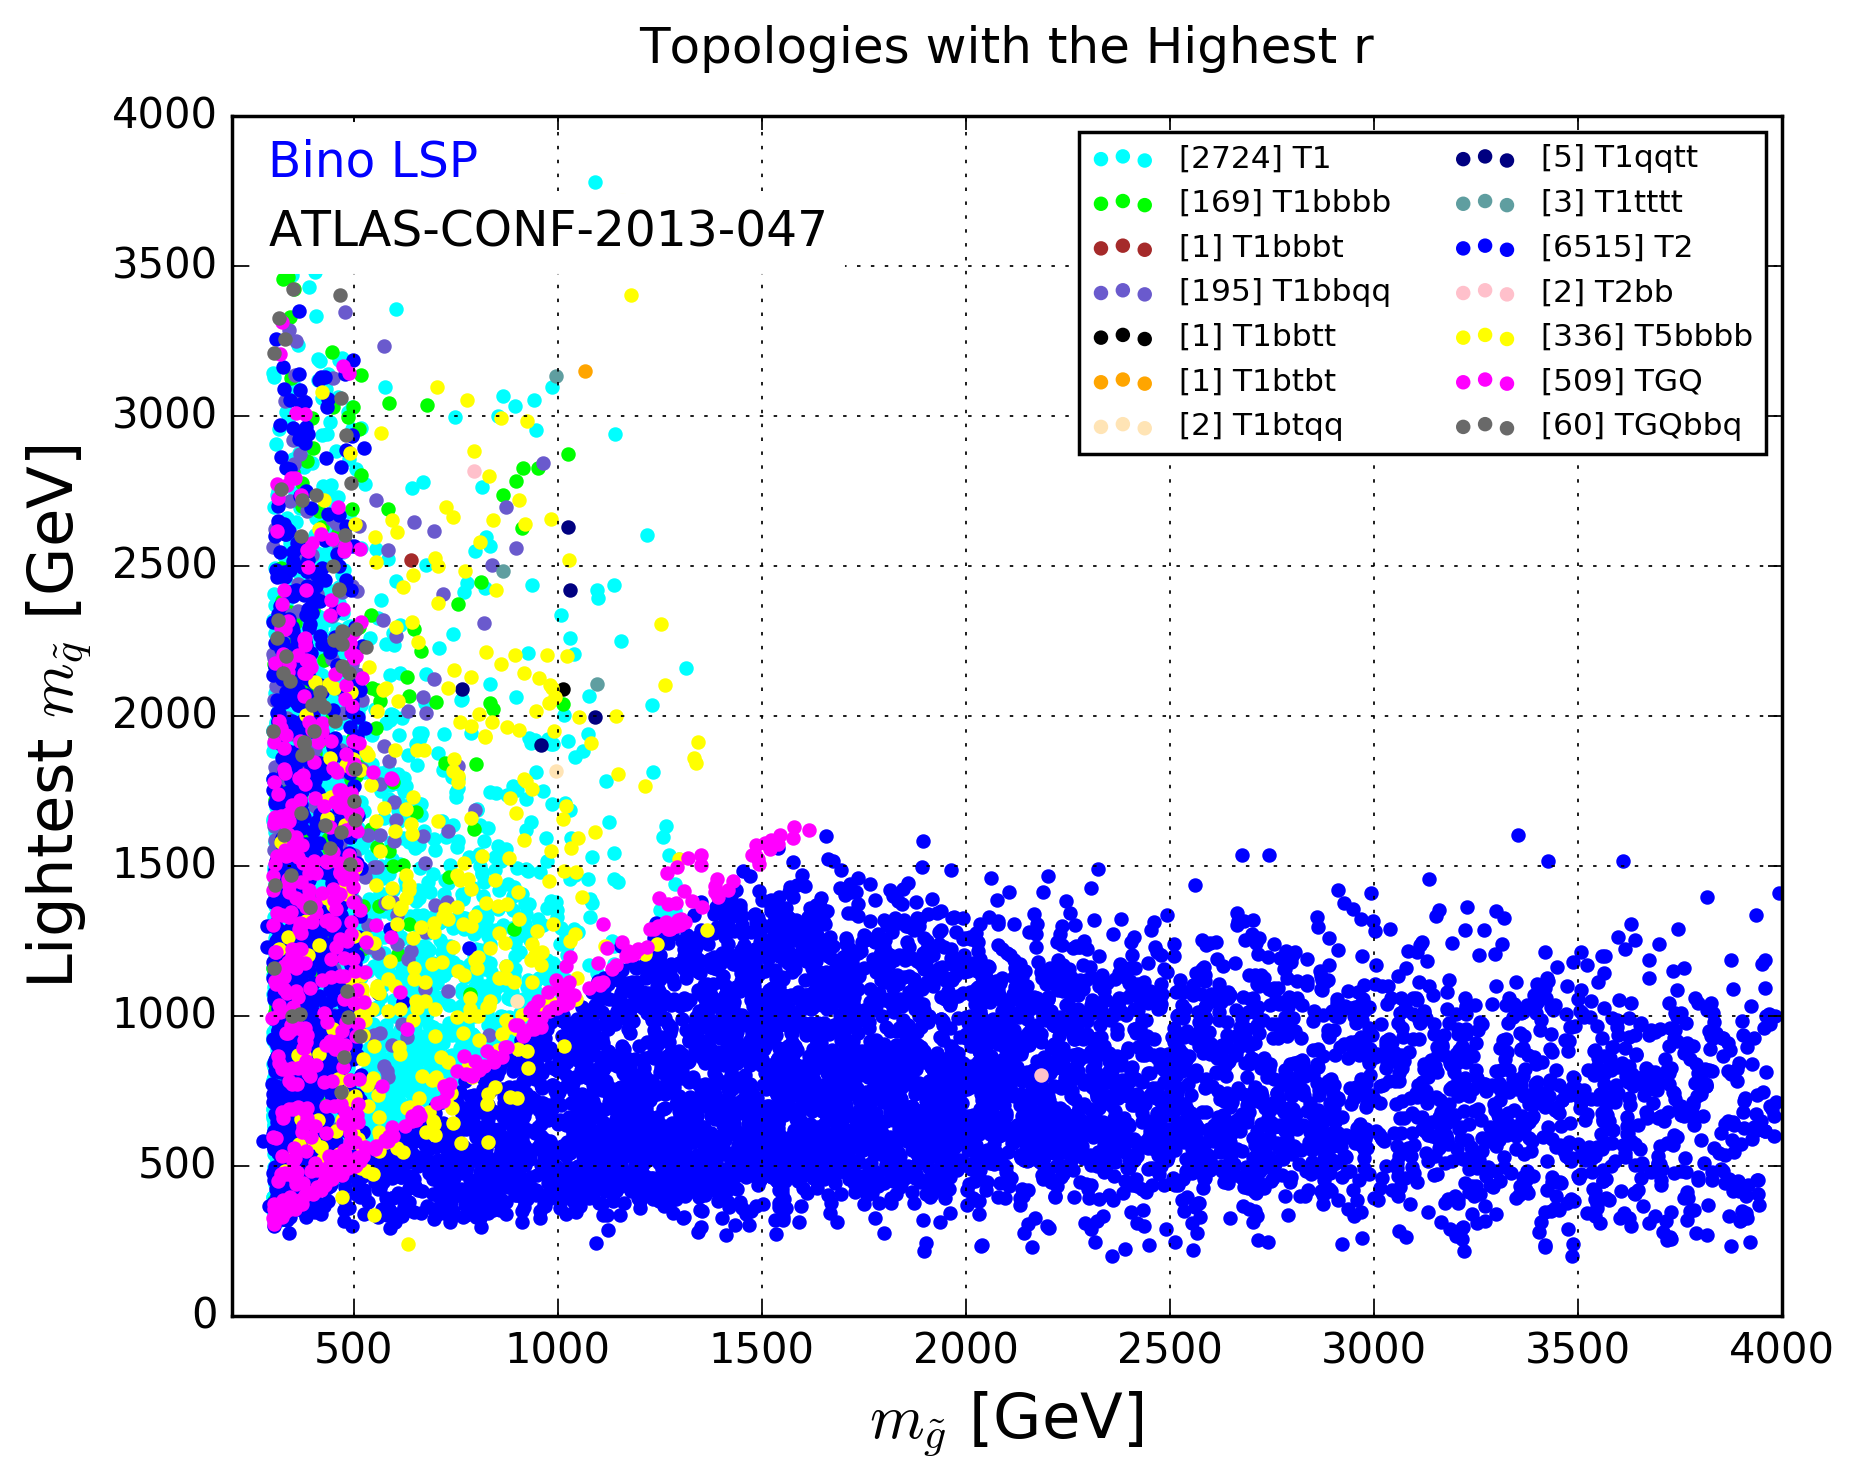
\includegraphics[width=0.49\textwidth]{Fig/FastLim/BinoTxNames_Scatter_Best_All_LightS_All.png}}
	\subfigure
	{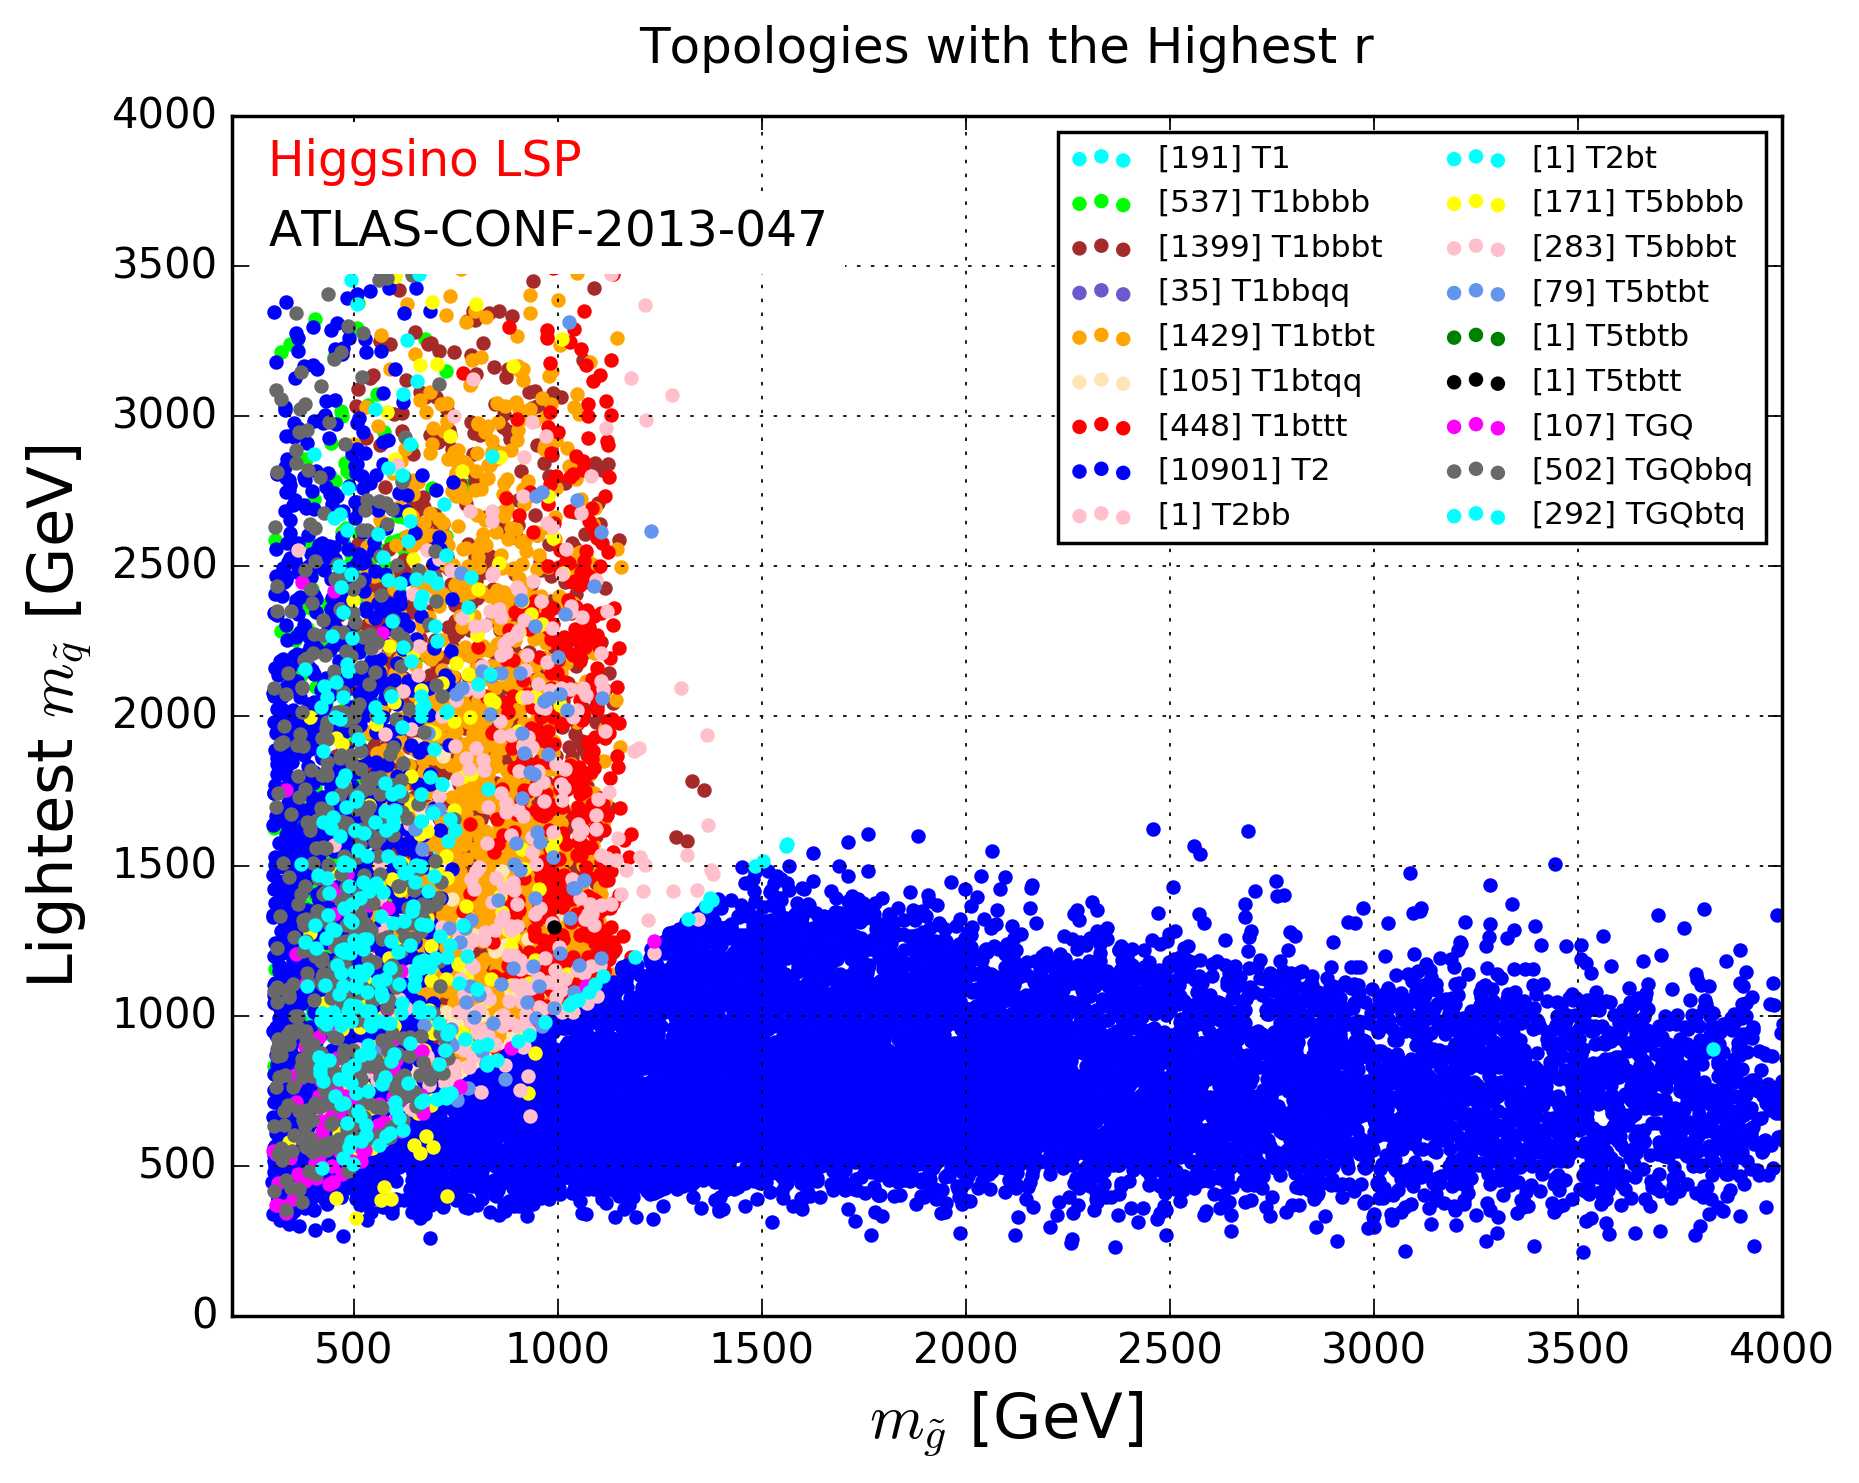
\includegraphics[width=0.49\textwidth]{Fig/FastLim/HiggsinoTxNames_Scatter_Best_All_LightS_All.png}}
	\subfigure
	{ 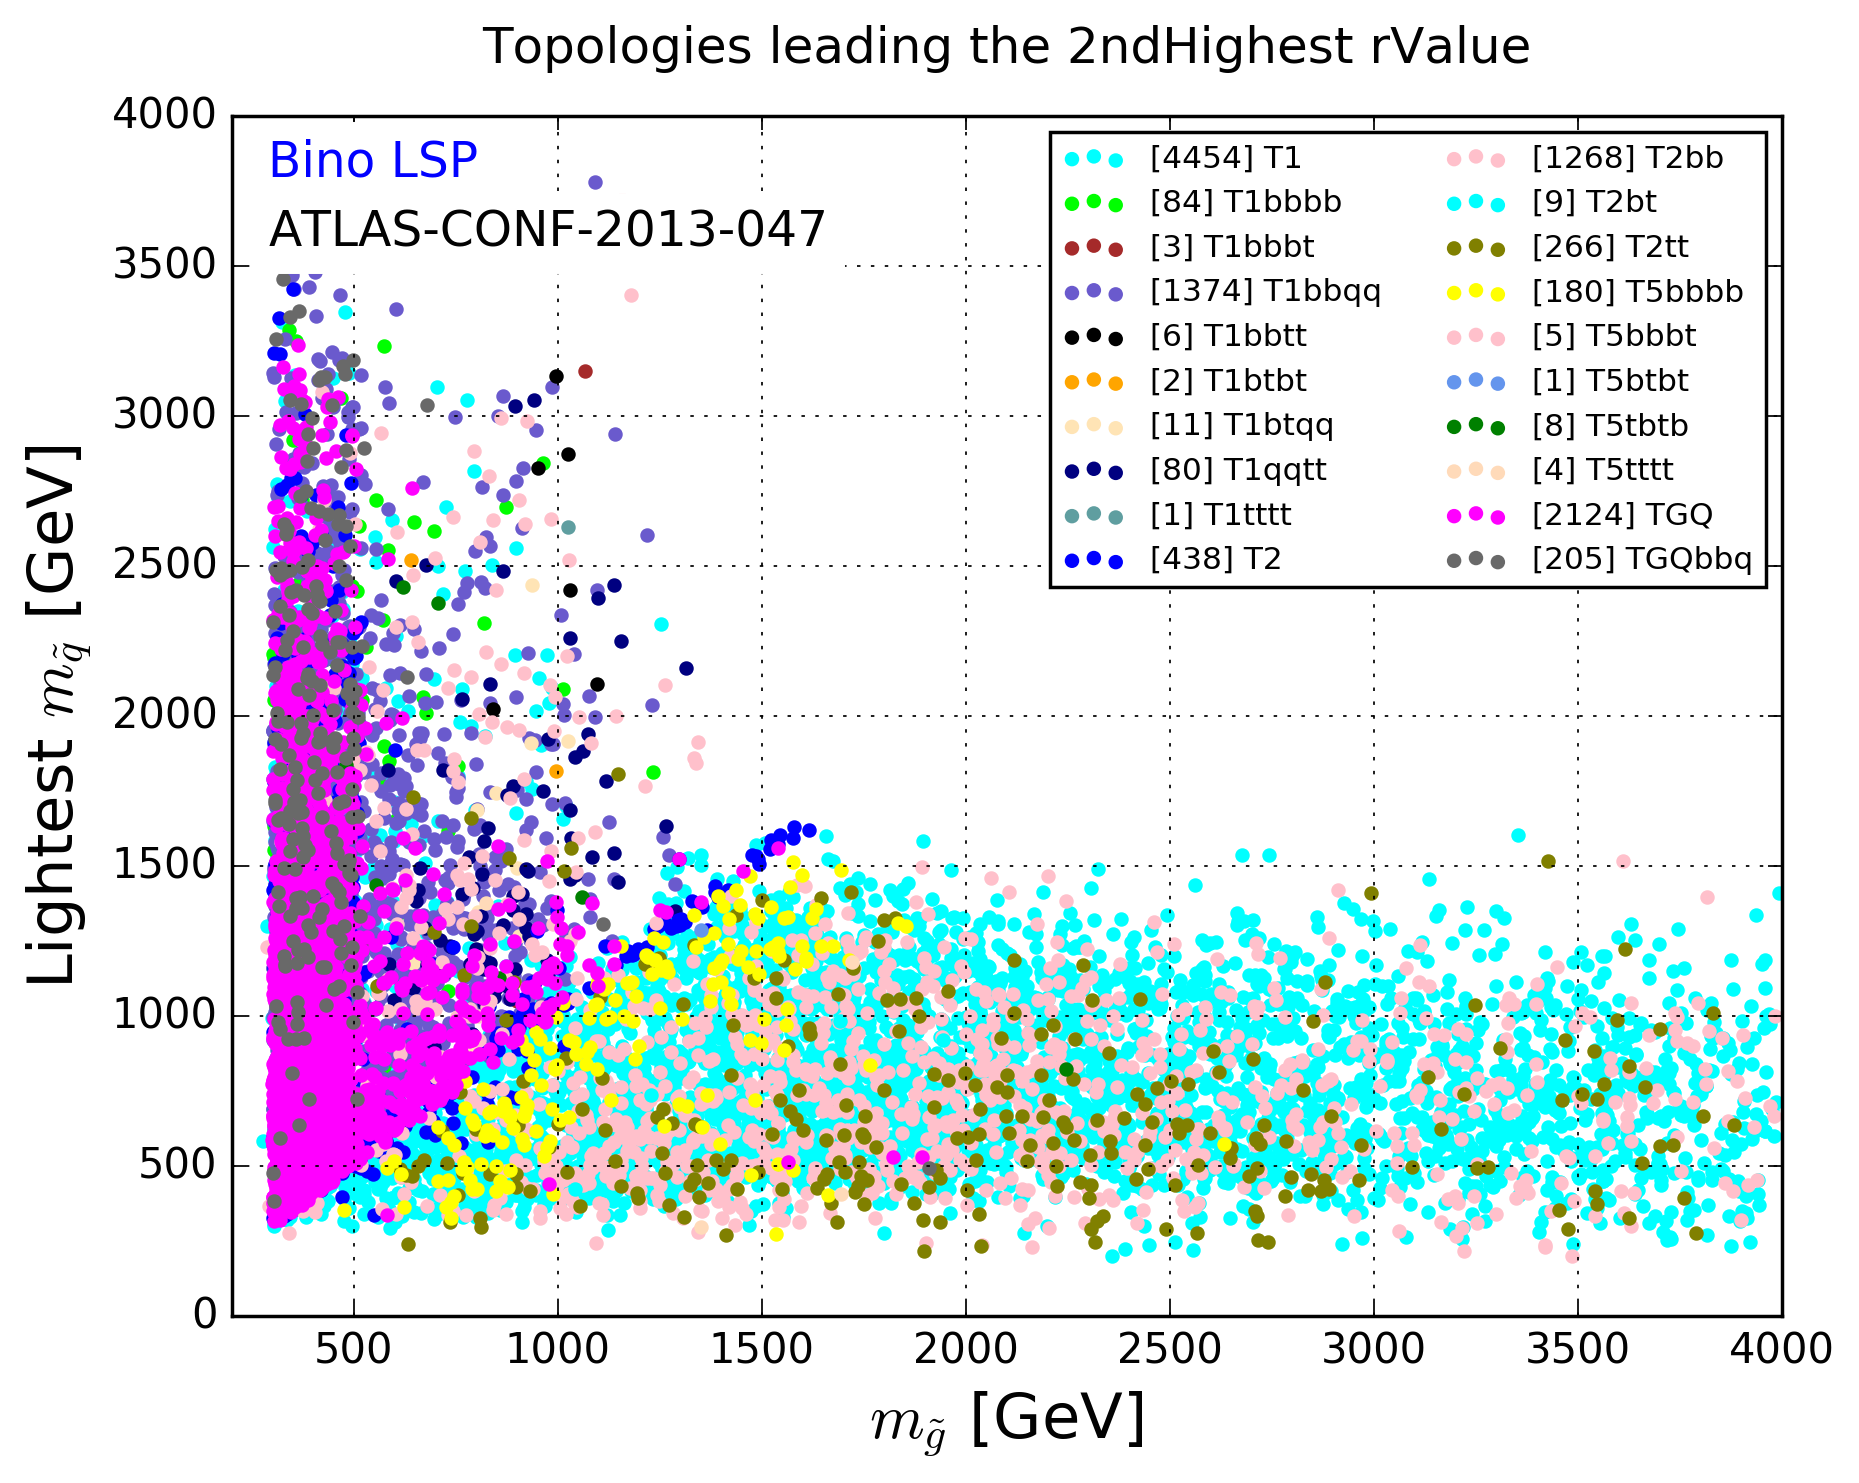
\includegraphics[width=0.49\textwidth]{Fig/FastLim/BinoTxNames_Scatter_2ndBest_All_LightS_All.png}}
	\subfigure
	{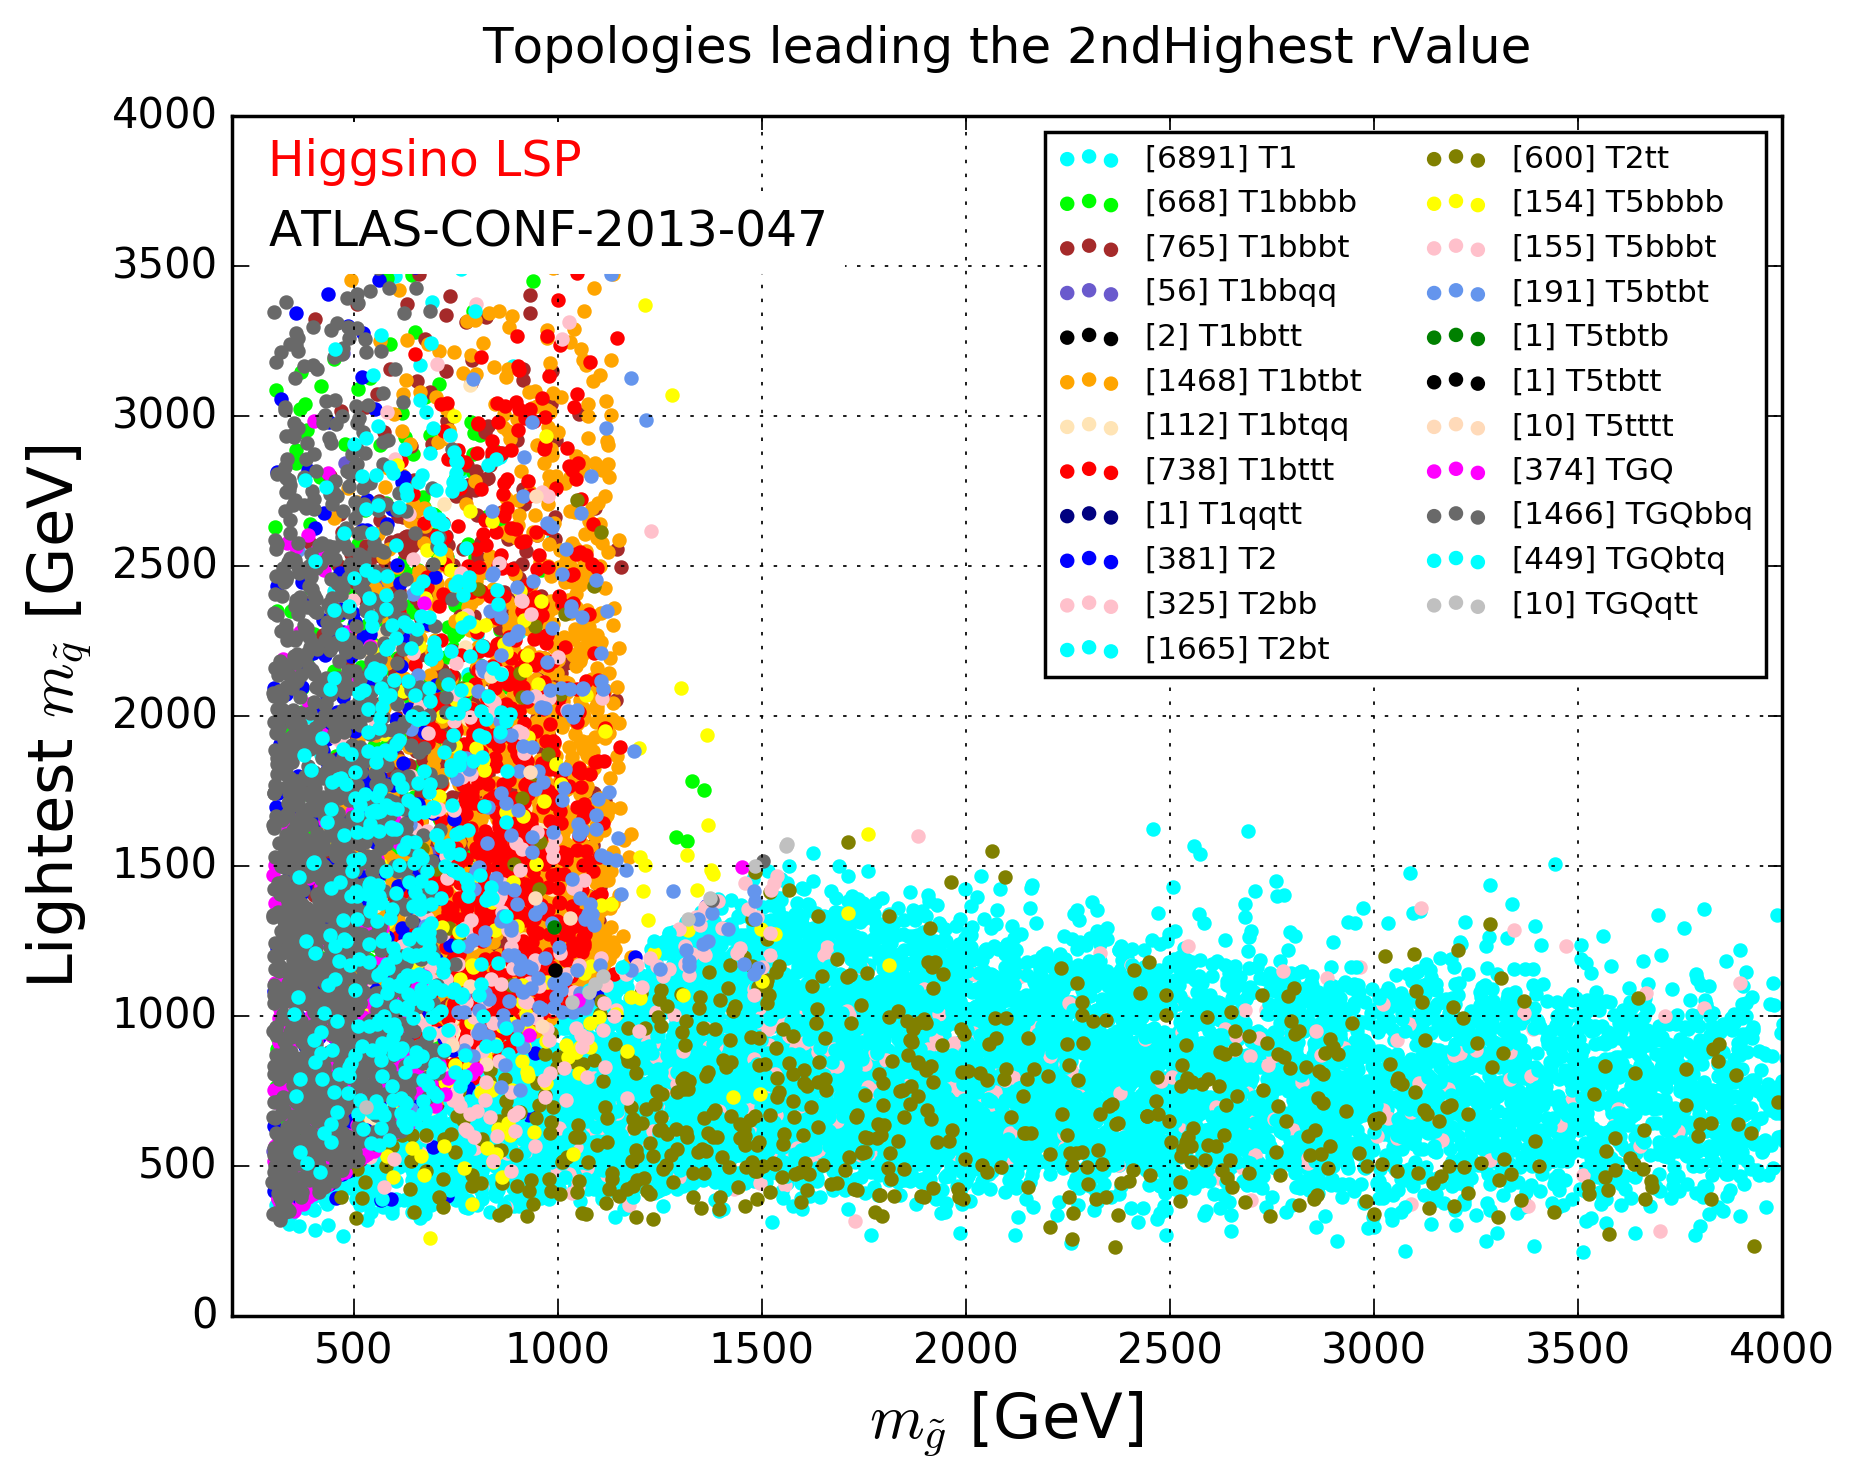
\includegraphics[width=0.49\textwidth]{Fig/FastLim/HiggsinoTxNames_Scatter_2ndBest_All_LightS_All.png}}
	\caption{Points excluded by \FastLim~ ATLAS-CONF-2013-047 results, with the color code indicating the topologies leading the best and 2nd-best r-value. Note that the points might be excluded by combination of different simplified models results, i.e. considering only one result might not be enough to get r-value$>$1. The number in the legend reports the total number of points considered for the particular simplified model. }
	\label{fastlim}
	
	
\end{figure}


\\

Conclusion: if I want to extend the results for the ATLAS-SUSY-2013-02 with new EMs results, aimign at combining as many signals as possible, it makes sense to start from this simplified models, since they carry the highest constraining power. 


\clearpage
\section{New results: T3GQ Maps}
\begin{figure}[!]
	\begin{center}
		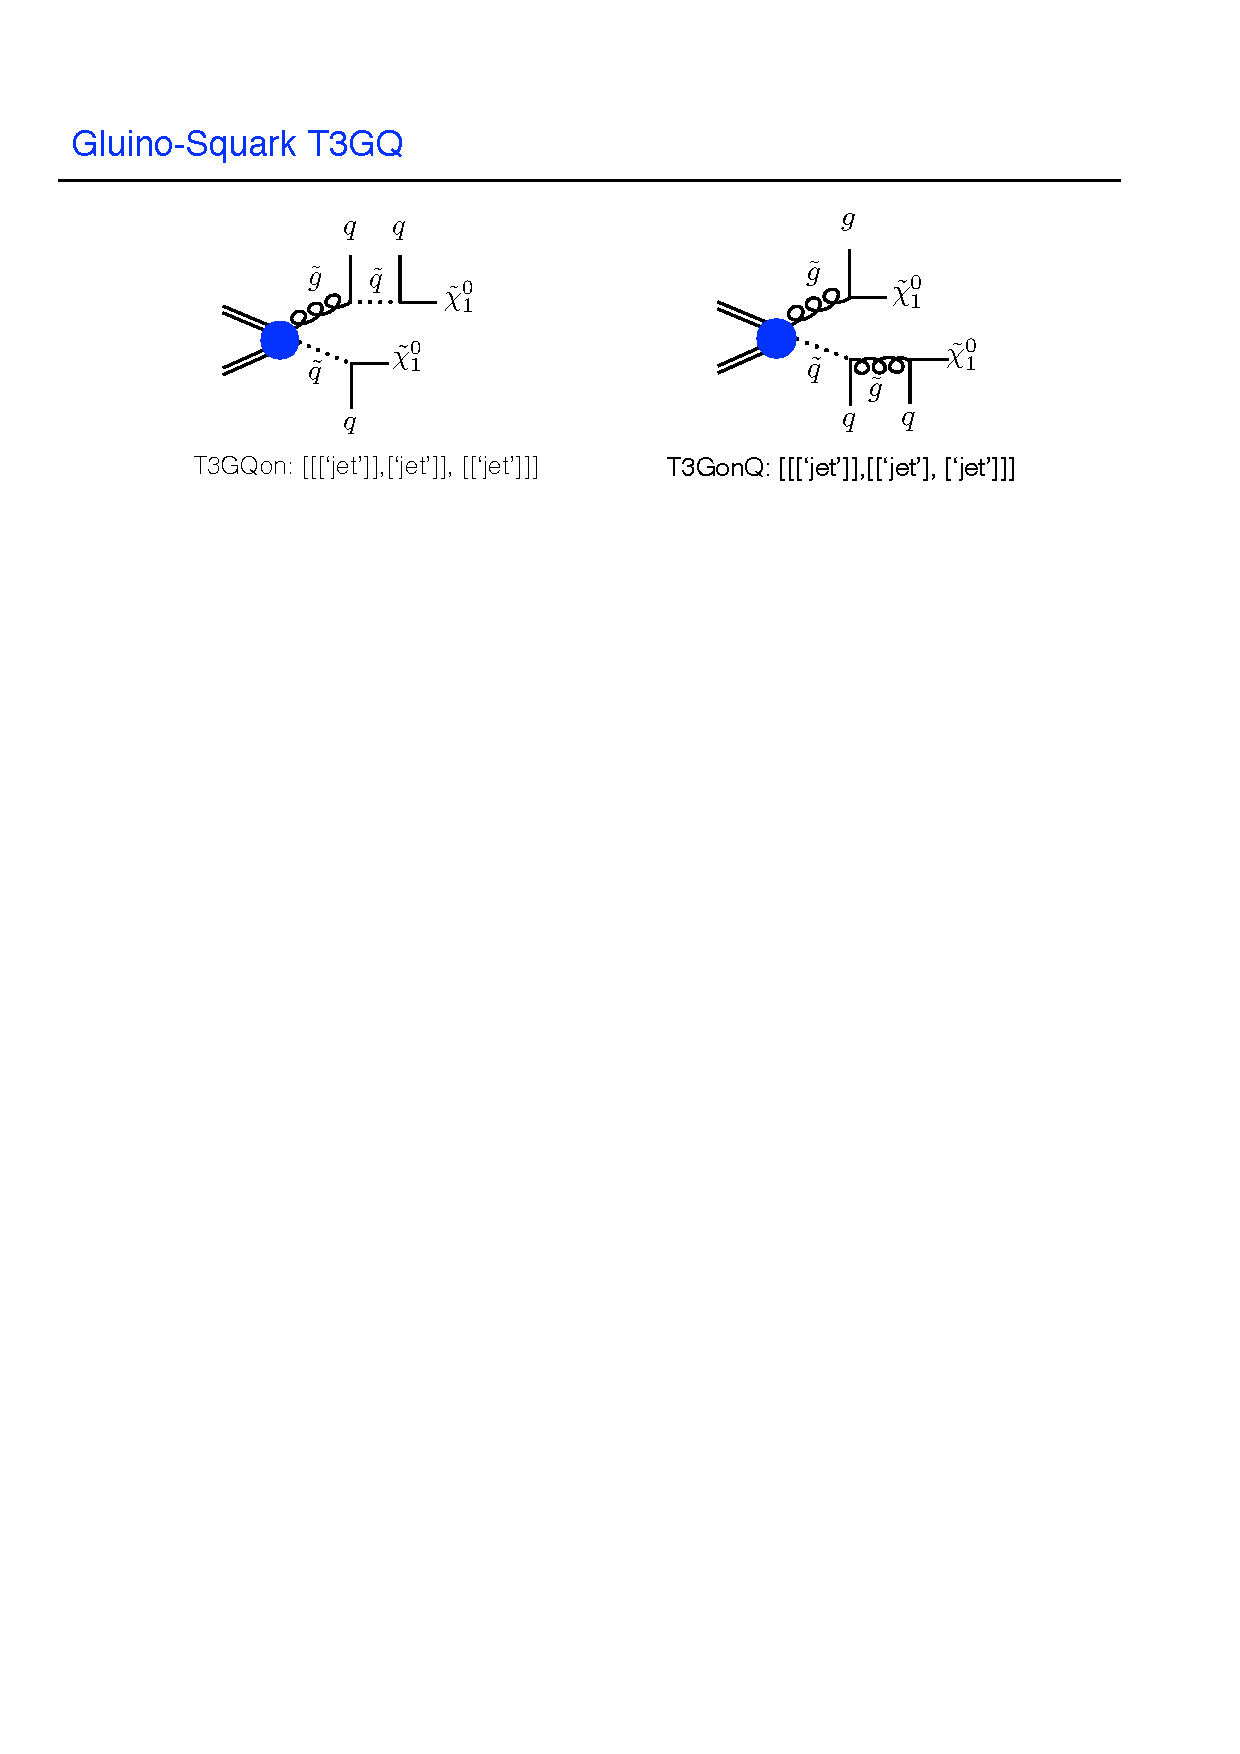
\includegraphics[width=0.8\textwidth]{Fig/TGQ/TGQ.pdf}
	\end{center}
	\caption{Diagrams for the T3GQ and T3QG simplified models.}
	\label{tgq}
\end{figure}

In this Section I discuss briefly the topic of "T3GQ" maps. As I pointed out in the \SMO~ paper Section, the main missing topology, at least by frequency of appearance in Fig. \ref{smo_paper_missing} for both Bino and Higgsino-LSP cases if defined by the [[jet]],[[jet][jet]] constraint, i.e. one jet from one branch, two jets from the other in two distinct vertices. Important to remember: \SMO~ does not generally distinguish between gluon and light quark jets, i.e. jet can be either a quark or a gluon (in the decomposition procedure). 
\\

It was tested that this particular signature can originate from gluino-squark production, which benefits of a very large production cross section at the LHC. There are two possible distinct cases where we can have this simplified model: either the gluino is heavier than the lightest squark, so that gluinos decay with basically 100$\%$ branching to on-shell intermediate squark, or the other way around, where this time the gluino is lighter that the lightest squark so that we will have a cascade decay with an on-shell intermediate gluino. The first case generates always (since all the other SUSY particles are neglected), a \jmet~ signature (see Fig. \ref{tgq}). The latter, only if the gluino loop-decays to gluon plus neutralino. If the mass splitting between the gluino and the lightest squark is small, however, you can also have a three-body decays to quark-antiquark-n1 via off-shell squark. 
\\


\begin{itemize}
\item I produced EMs results for the T3GQ model (which in \SMO> assumptions apply also to the T3QG case)
for the ATLAS-SUSY-201-02 and CMS-SUS-13-012 "all-hadronic", 0-lepton final states searches
\item I rerun the scan and checked any improvement. Results are in Fig.\ref{improved}
\end{itemize}




\begin{figure}[!b]
	\centering
	\subfigure
	{ 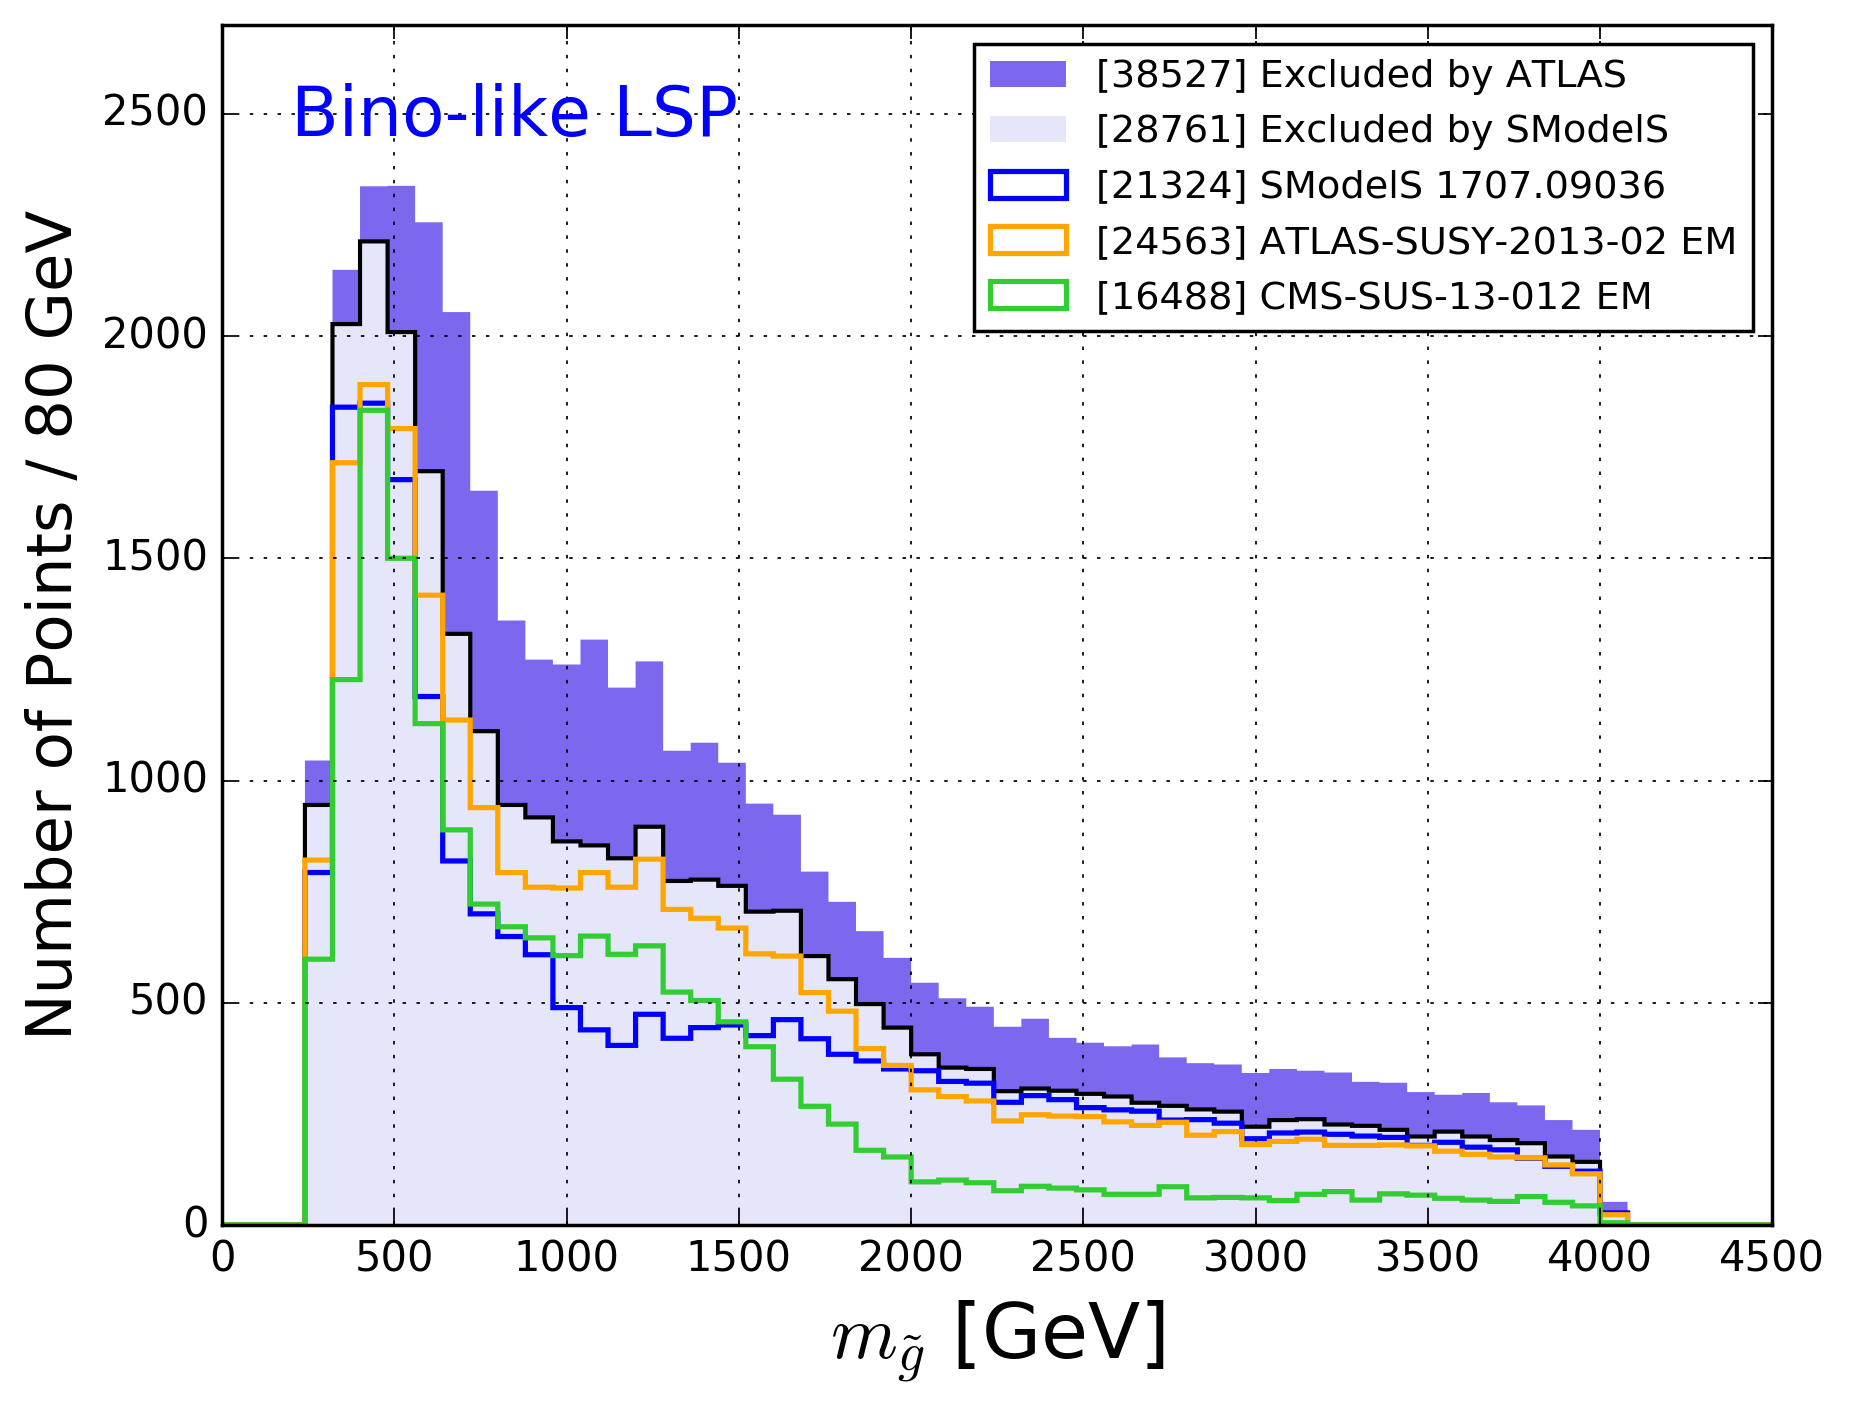
\includegraphics[width=0.49\textwidth]{Fig/TGQ/Bino_TOTAL_COMPARISONOLD_Histo.png}}
	\subfigure
	{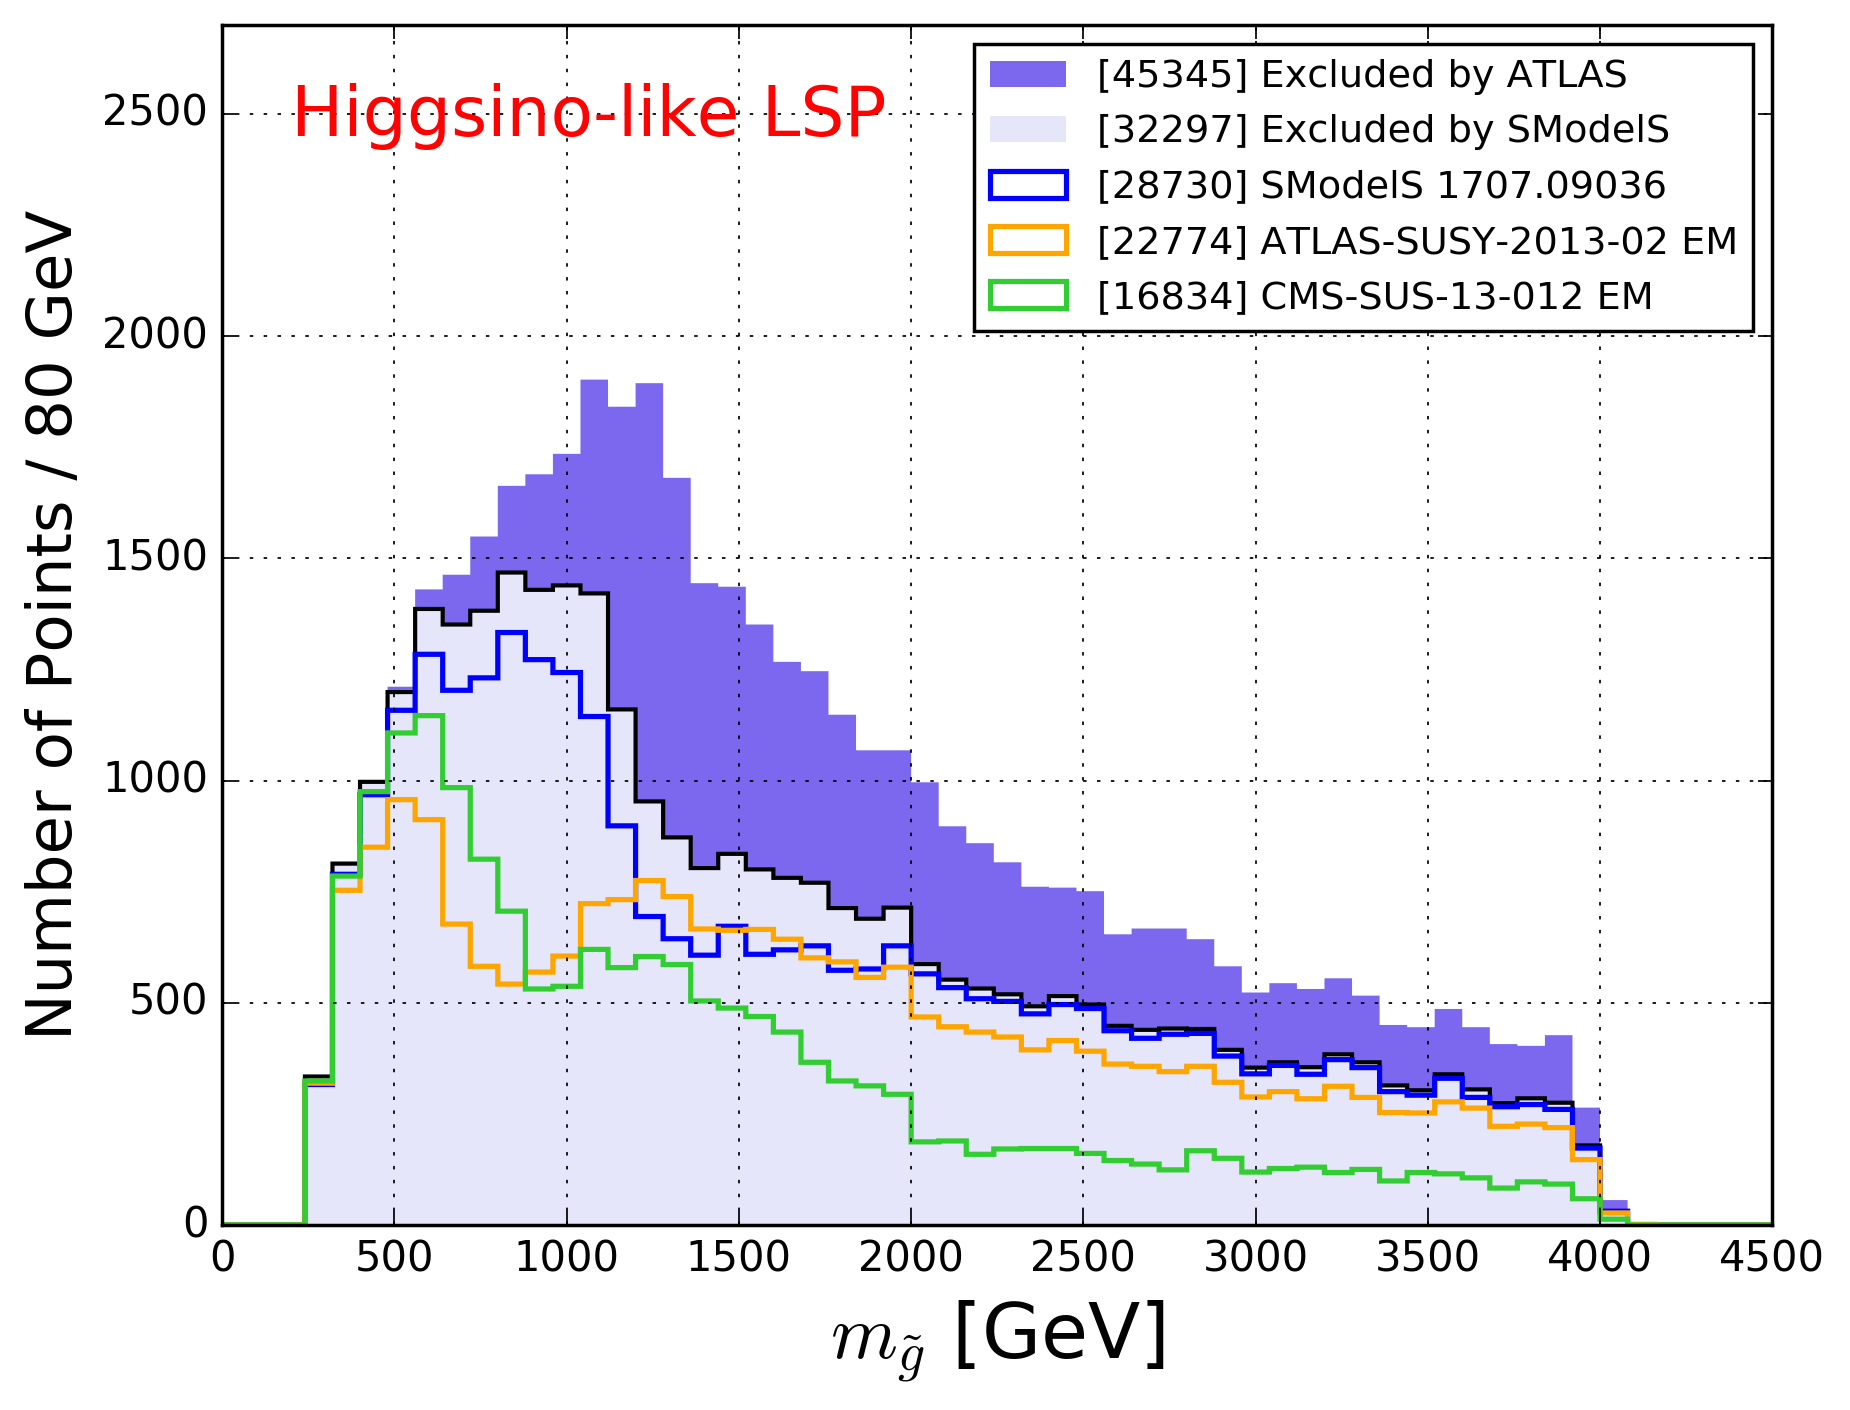
\includegraphics[width=0.49\textwidth]{Fig/TGQ/Higgsino_TOTAL_COMPARISONOLD_Histo.png}}
	\caption{Improved constraints (on the same Bino - Higgsino like LSP datasets) coming from the addition of the T3GQ EMs.}
\label{improved}
\end{figure}



Fig. \ref{tgq} shows the possible diagrams that lead to the \jmet~ signature, from gluino-squark associated production decaying according to the two possible mass hierarchies.


\clearpage
\section{Results}
In this Section I summarize briefly the results from the first, preliminary scan of points that Bjorn provided.
\subsection{Mass Distributions}
In Fig. \ref{masses} the distributions of the masses of the scanned points are shown; in particular, all the coloured particles have very large masses exceeding 2 TeV, so that essentially only electroweak productions have reasonable cross sections.
This configuration of mass parameters is very challenging for \SMO~, since basically EMs for squark are produced up to around 1 TeV, and gluino EMs for up to 1.5 TeV (but cross sections should be very small in any case to contribute significantly). 
\\
Concerning the Electroweak simplified models, they are very poorly covered: only TSlepSlep (slepton production and direct decay) and TChiWZ (chargino-neutralino2 production but strictly mass degenerate ) are essentially covered. 

\begin{figure}[!b]
	\centering
	\subfigure
	{ 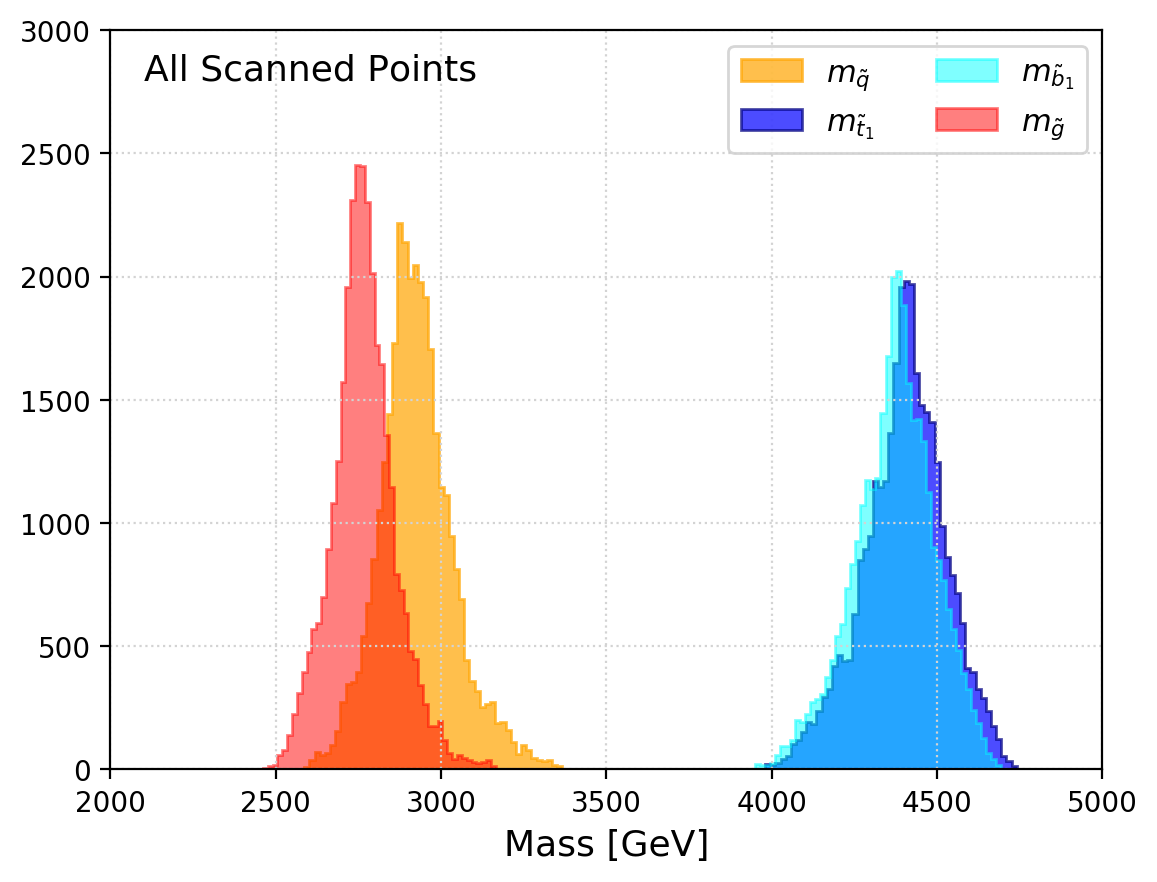
\includegraphics[width=0.49\textwidth]{Fig/Res/Coloured.png}}
	\subfigure
	{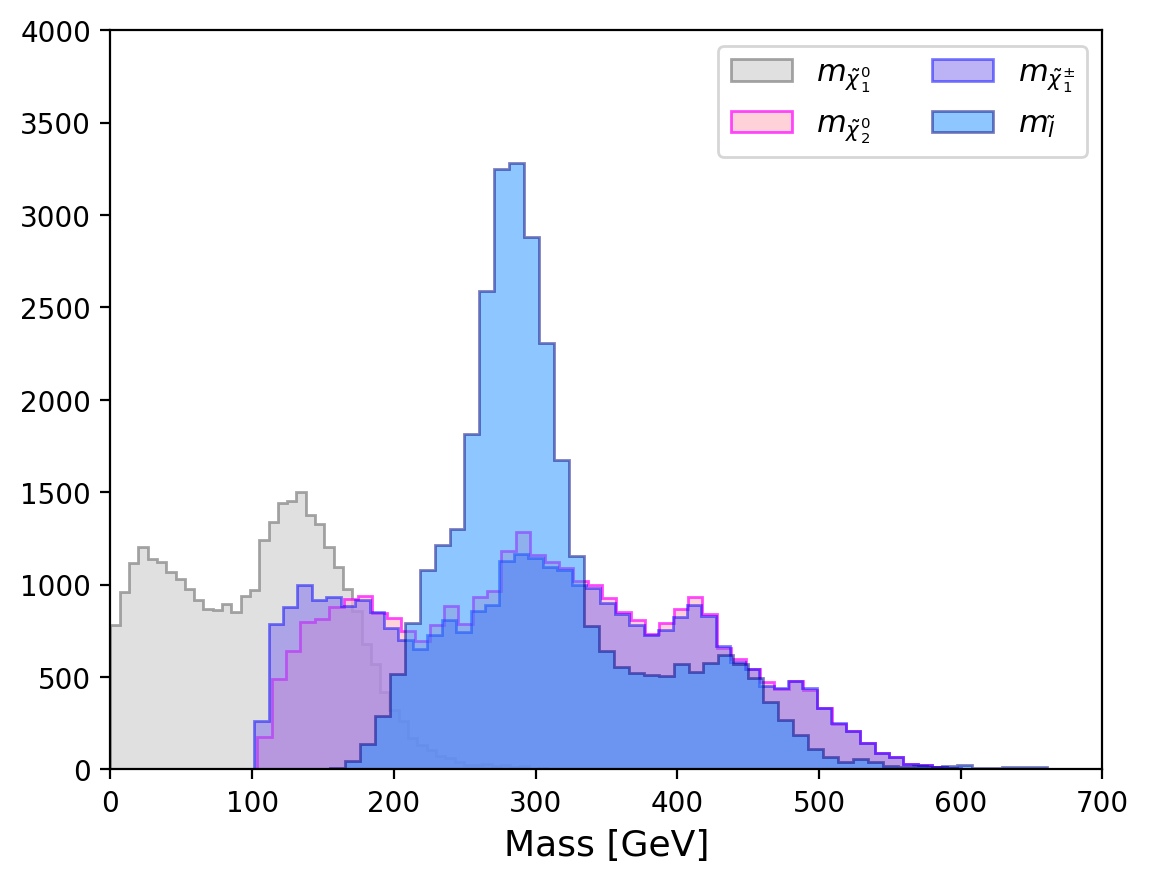
\includegraphics[width=0.49\textwidth]{Fig/Res/EW.png}}
	\subfigure
    {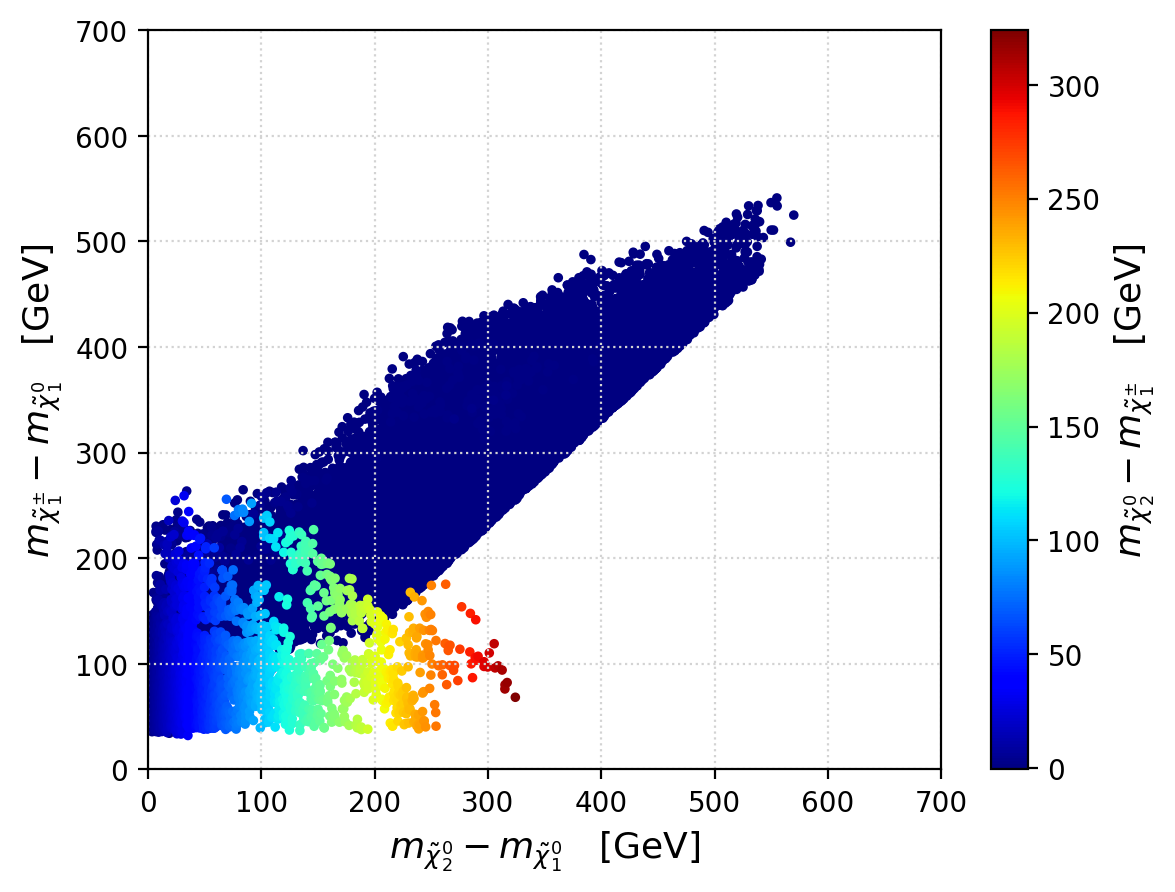
\includegraphics[width=0.49\textwidth]{Fig/Res/Diff_EW.png}}	
	\caption{Distributions of the masses of the SUSY particles of the first set of points.}
	\label{masses}
\end{figure}

\clearpage
\subsection{Missing TxNames and Missing Brackets}
Here I list the most frequent (at least $> 100$ times) missing TxNames and missing brackets, with the largest weight ($\sigma \times BR$) for each point. I am not sure about the interpretation of the two definitions, so I hope Bjorn will clarify this.

\begin{verbatim}
('TChiChipmhiggs_W_', 136)
('TChiChipmZW_WW_', 144)
('TChiChipmqq_W_', 166)
('', 401)
('TChiChipm__', 540)
('TChiChipmmu__', 639)
('TChipChimWoff_Woff_', 950)
('TChiChipm_Woff_', 1341)
('TChiChipmZoff_Woff_', 1569)
('TSnuSnu__', 3249)
('TChiChipm_W_', 3621)
('TChiChi__', 5481)
('TChiChipme__', 8087)
\end{verbatim}

\begin{verbatim}
('[[[W],[W]],[[Z],[W]]]', 160)
('[[[jet,jet]],[[photon]]]', 176)
('[[],[[l,nu]]]', 179)
('[[[W]],[[jet,jet]]]', 184)
('', 401)
('[[],[[W]]]', 1431)
('[[],[[jet,jet]]]', 1648)
('[[[jet,jet]],[[l,nu]]]', 1856)
('[[[W]],[[l,nu]]]', 2124)
('[[],[]]', 4794)
('[[],[[l]]]', 13435)
\end{verbatim}

There are some things that I cannot explain, e.g.
\begin{itemize}
	\item The difference between 'TChiChipme' and the '[[],[[l]]]' constraint? Are those referring to the same topology? \\
	\item Why "TChiChipmmu" is much less frequent than "TChiChipme"? 
	\item What is "TSnuSnu" ?
\end{itemize}


  



\clearpage
\section{Efficiency Maps Production}
In Tab. \ref{EM} the overview of the EMs produced for the analysis ATLAS-SUSY-2013-02 is given. 
\begin{table*}[!h]
\centering
\renewcommand{\arraystretch}{1.2}
\small
\begin{tabular}{ l  c } \toprule \toprule 
	
\textbf{Model} & \textbf{Mass Plane} \\ \toprule \toprule 
\multicolumn{2}{c}{\textbf{Squark}}  \\ \hline
T2 & - \\
\multicolumn{2}{c}{\textbf{3rd Generation}}  \\ \hline
T2bb & - \\
T2tt & - \\
T2bt & - \\

\multicolumn{2}{c}{\textbf{Gluino-Squark}}  \\ \hline
T3GQ & - \\

\multicolumn{2}{c}{\textbf{Gluino} }  \\ \hline
T1qqqq (Off.) & - \\
T1bbbb & - \\
T1btbt & - \\

T3GGgbb & - \\
T3GGgqq & - \\
T5(qqqq) & - \\
T5bbbb & $x=(0.05, 0.50, 0.95)$ \\

\multicolumn{2}{c}{\textbf{Electroweak} } \\ \hline
TChiW & - 

    \bottomrule 
  \end{tabular}
  \caption{Summary of EMs results for the analysis ATLAS-SUSY-2013-02. "Off" stands for official result (from the ATLAS Coll.).}
  \label{EM}
\end{table*}

Using the information from Section \ref{ATLAS047}, the most useful EMs to be produced for the analysis ATLAS-SUSY-2013-02 should be:
\begin{itemize}
	\item T1bbqq (almost finished) \
	\item T1bbbt \
	\item T1btqq \
	\item T1bttt \
	\item T3GGbtq (aka TGQbtq) \
	\item T5bbbt \
	\item T5btbt \
\end{itemize}
\\

Going to the following most important missing topologies from Fig. \ref{smo_paper_missing}, the other gluino-squark models after the T3GQ which is already done, are the ones giving the "[[jet][jet,jet]][[jet,jet]]" (Higgsino) and "[[jet]][[jet][jet,jet]]"(Bino) models. I believe these are the most important models to produce, however they will take a lot more time since they depend on three free parameters and the cross section is large even for large masses (e.g. heavy gluino-light squark) .
\\

About the "[[]],[[jet,jet]]", which I call TGN: it can come from gluino-neutralino or pure electroweak processes. I have produced the maps for the model already, considering the gluino-neutralino case. Even though they will apply also to the EW case, I am not sure how valid is the simplified model assumption in this case (e.g. how much it depends on ISR?). Maybe it is a good test case.
Also note that this topology is basically the off-shell version of the TChiW model "[[]],[[W]]". 
%
\section{Extra EMs results}
In the following tables, EMs for other simplified models (with focus on third generation squarks) that I produced in the past and never used in publications are listed. They were mostly produced for the analysis CMS-SUS-13-012, which however is less constraining than ATLAS-SUSY-2013-02 due to the presence of 36 non overlapping signal regions, so they prove sensitive only to specific signals and it is hard to take advantage of signal combination with EMs results. However they cover a large fraction of scenarios like natural SUSY. I could not really test them with the ATLAS pMSSM scan since all the 3rd generation squarks were quite heavy.
\\

It will make sense to re-produce them for ATLAS-02 as well. In particular, simplified models with Higgs decays should be important. In the past I was warned that generation of such models is tricky because of how the Higgs mass was handled by Pythia (???), but the person who told me that could not elaborate why (???). 

\begin{table}\centering\footnotesize
	\renewcommand{\arraystretch}{1.5}
	\begin{tabular}{ l | l  l  l  c } 
		\multicolumn{5}{c}{\large \textbf{Additional Recast Results}} 
		\\ 
		\toprule \toprule 
		\textbf{Process} & \textbf{Txname} & \textbf{Decay} & \textbf{Mass Plane} & \textbf{Analyses} \\ \toprule \toprule
		$p p \rightarrow \tilde g \tilde g $ & T5WW   & $\tilde g \rightarrow q \bar{q}' \tilde \chi^{\pm}_1$, $\tilde \chi^{\pm}_1 \rightarrow W^\pm \tilde \chi^0_1$ & $x = (0.25)$ & [1] \\ \midrule
		
		$p p \rightarrow \tilde q \tilde q^* $ & T6WW & $ \tilde q \rightarrow q' \tilde\chi^{\pm}_1$ ,   $ \tilde\chi^{\pm}_1 \rightarrow W \tilde\chi^{0}_1$ &  $x=(0.50,0.95)$ & [1] \\
		$[\tilde q = (\tilde u, \tilde d, \tilde c, \tilde s)_{L,R}]$ & & & $\Delta M(\tilde\chi^\pm_1,\tilde\chi^0_1) = (5,40,75)$ GeV & \\ \midrule
		
		% ***************** sbottoms
		$p p \rightarrow \tilde b_1 \tilde b_1^*$ & T6bbZZ & $\tilde b_1 \rightarrow b \tilde\chi^0_2$, $\tilde \chi ^0 _2 \rightarrow Z \tilde \chi^0_1$ & $x =(0.25,0.50,0.95)$  & [1] \\
		& & & $\Delta M(\tilde\chi ^0_2,\tilde\chi^0_1)=(5,50,75)$ GeV & \\ 
		
		& T6WWtt & $\tilde b_1 \rightarrow t \tilde\chi ^{\pm} _1$, $\tilde\chi ^{\pm} _1 \rightarrow W \tilde \chi^0_1$ & $x =(0.25,0.50,0.75)$  & [1] \\
		& & & $\Delta M(\tilde b_1,\tilde t_1)=(5,40,75)$ GeV & \\ 
		& & & $\Delta M(\tilde t_1,\tilde \chi ^0_1)=(90,130,165)$ GeV & \\ 
		
		& T6ttWW & $\tilde b_1 \rightarrow W \tilde t_1$, $\tilde t _1 \rightarrow t \tilde \chi^0_1$ & $x =(0.25,0.50,0.75)$  & [1] \\
		& & & $\Delta M(\tilde b_1, \tilde \chi_1 ^{\pm})=(130,165)$ GeV & \\ \midrule
		& & & $\Delta M(\tilde \chi_1^{\pm}, \tilde \chi_1 ^0)=(5,40,75)$ GeV & \\ \midrule
		
		
		% ***
		$p p \rightarrow \tilde b_2 \tilde b_2^*$ & T6ZZbb & $\tilde b_2 \rightarrow Z \tilde b_1$, $\tilde b_1 \rightarrow b \tilde \chi^0_1$ & $x =(0.10,0.50,0.95)$  & [1] \\
		& & & $\Delta M(\tilde b_2,\tilde b_1)=(5,50,75)$ GeV & \\   \midrule
		
		% ***************** stop
		$p p \rightarrow \tilde t_1 \tilde t_1^*$  & T6ttZZ & $\tilde t_1 \rightarrow t \tilde\chi_2 ^0$, $\tilde \chi_2 ^0 \rightarrow Z \tilde \chi^0_1$ & $x =(0.50,0.70)$  & [1] \\
		& & & $\Delta M(\tilde \chi_2^{0}, \tilde \chi_1 ^0)=(5,45,85)$ GeV & \\ 
		& & & $\Delta M(\tilde t_1, \tilde \chi_2 ^0)=(200)$ GeV & \\ 
		
		& T6WWbb & $\tilde t_1 \rightarrow W \tilde b_1 $, $\tilde b_1 \rightarrow b \tilde \chi^0_1$ & $x =(0.05,0.50,0.75)$  & [1] \\
		& & & $\Delta M(\tilde b_1, \tilde \chi_1 ^0)=5$ GeV & \\ 
		& & & $\Delta M(\tilde t_1, \tilde b_1 )=(10,40,75)$ GeV & \\ \midrule
		
		$p p \rightarrow \tilde t_2 \tilde t_2^*$ & T6ZZtt & $\tilde t_2 \rightarrow Z \tilde t_1$, $\tilde t_1 \rightarrow t \tilde \chi^0_1$ & $x =(0.10,0.50,0.95)$  & [1] \\
		& & & $\Delta M(\tilde t_2,\tilde t_1)=(5,40,80)$ GeV & \\ 
		& & & $\Delta M(\tilde t_1,\chi^0_1)=(90,160)$ GeV & \\ \midrule
		
		$p p \rightarrow \tilde l^+ \tilde l^-$ & TSlepSlepWW & $  \tilde l ^{\pm}  \rightarrow \chi _1^{\pm}$, $ \chi _1^{\pm} \rightarrow W^{\pm} \tilde\chi^0_1$ & $x=(0.2,0.50,0.90)$ & [1],[4],[5]  \\
		& & 																			& $\Delta M(\tilde\chi^\pm_1,\tilde\chi^0_1) = (10,40,75)$ GeV            & \\ \midrule
		$p p \rightarrow \tilde g  \tilde \chi _1 ^0$ & TGN & $\tilde g \rightarrow q \bar q \chi _1 ^ 0$ & -  & [1],[5] \\ 
		\bottomrule \bottomrule
	\end{tabular}
	\caption{Additional unpublished EM results.[1]: CMS-SUS-13-012 (MA5) , [2]: ATLAS-SUSY-2013-04 (MA5), [4]: ATLAS-SUSY-2013-11 (MA5).} 
	\label{extra_sms}
\end{table}



\section*{Acknowledgments}
Thanks!
%
\bibliographystyle{JHEP}
\bibliography{references}

\end{document}
